\documentclass[xcolor=table]{beamer}
\usetheme[progressbar=frametitle]{metropolis}
\usepackage{appendixnumberbeamer}

\usepackage[absolute,overlay]{textpos}
\usepackage{booktabs}
\usepackage{pgf, tikz}
\usepackage{pdfcomment}
\usepackage{pgfplots}
\usepackage{hyperref}
\usepackage[utf8]{inputenc}
\usepackage{xspace}
\usepackage{color}
\newcommand{\themename}{\textbf{\textsc{metropolis}}\xspace}
\newcommand\FontImportant{\fontsize{15}{20}\selectfont}
\newcommand\FontMoyenImportant{\fontsize{14}{17}\selectfont}
\newcommand\FontPetit{\fontsize{8}{6}\selectfont}
\title{Simulation de formes réalistes de développement résidentiel, de l'échelle du bâtiment à celle de l'ensemble d'une région urbaine}
\author{Maxime Colomb}
\subtitle{\textit{Sous la direction de M. Brasebin, J. Perret \& C. Tannier}
	\\Soutenance de thèse}

\titlegraphic{
\includegraphics[height=1.1cm]{Images/logoIGN.png}\hfill
\includegraphics[height=1.1cm]{Images/logoThema.jpg}}

\makeatletter
\newcommand\addsectiontotoc[1]{%
  \addtocontents{toc}{%
    \protect\beamer@sectionintoc{\the\c@section}{#1}{\the\c@page}{\the\c@part}%
                                {\the\beamer@tocsectionnumber}}
}
\makeatother

\makeatletter
\newcommand{\miniscule}{\@setfontsize\miniscule{4}{5}}% \tiny: 5/6
\makeatother

\setbeamerfont*{section in head/foot}{size=\miniscule}
\setbeamercolor{section in head/foot}{parent=palette primary}

\addtobeamertemplate{frametitle}{}{%
  \begin{textblock*}{5cm}(11cm,0.1cm)
    \insertsectionnavigation{4cm}
  \end{textblock*}
}
\begin{document}

\maketitle
\section{Introduction}
\begin{frame}{Contexte : le phénomène d'étalement urbain}
	\begin{block}{}
		\begin{itemize}
			\item Répond aux souhaits d'un grand nombre de ménages
			\item Multiples effets négatifs
			\item Objectif de régulation des pouvoirs publics
		\end{itemize}
		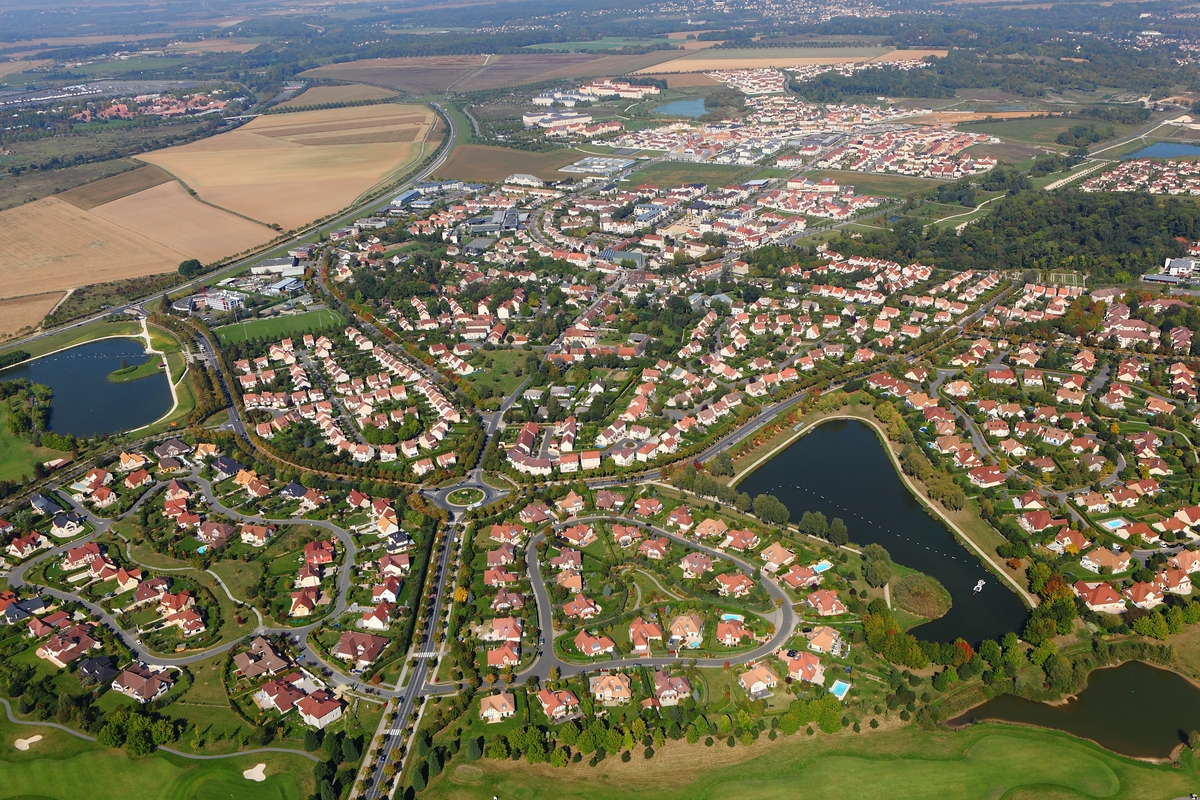
\includegraphics[height=2.8cm]{Images/consome.jpg}
		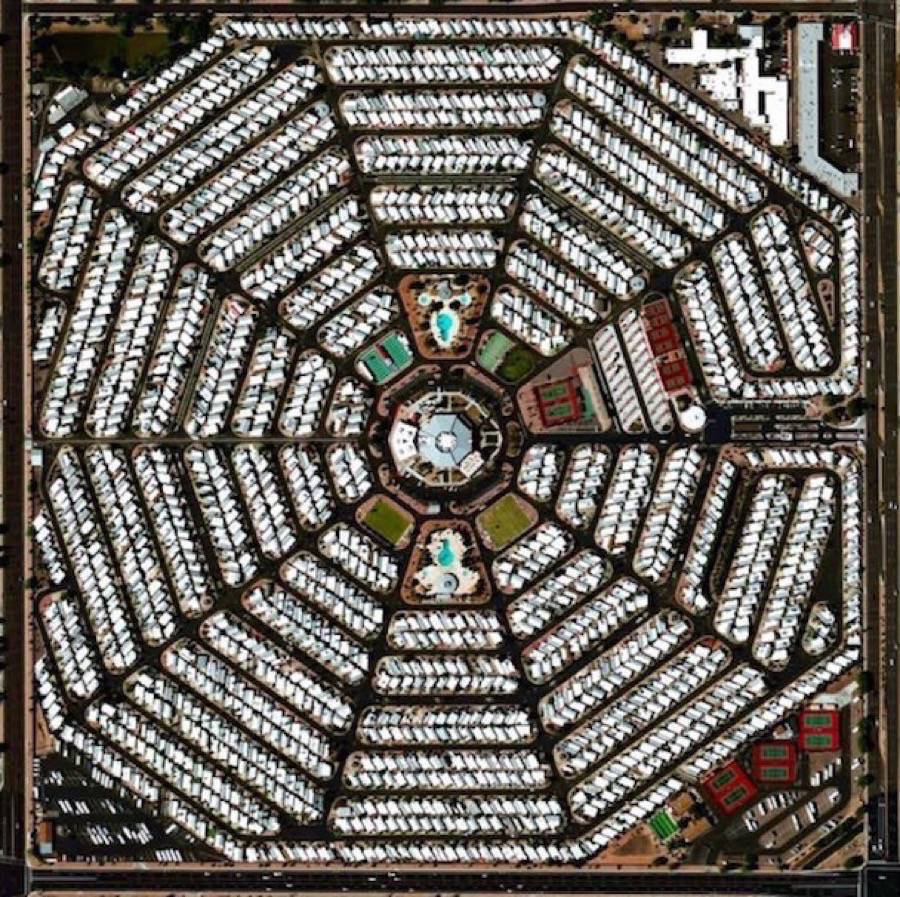
\includegraphics[height=2.8cm]{Images/sto.jpeg}
	\end{block}
	\begin{block}{}
		Dynamiques résidentielles prépondérantes %Le logement étant le principal levier de ce développement, nous nous concentrons sur le développement résidentiel
	\end{block}
\end{frame}

\begin{frame}{Contexte : documents d'aménagement réglementant l'extension résidentielle} 
	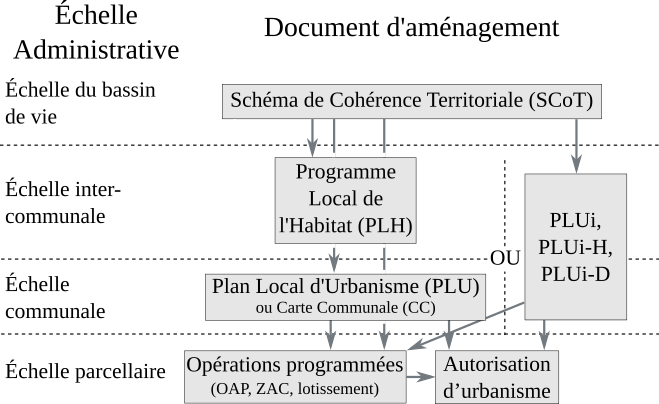
\includegraphics[width=11cm]{Images/planification-globale-Prez.png}
\end{frame}

\begin{frame}{Différents types de contraintes réglementaires} 
	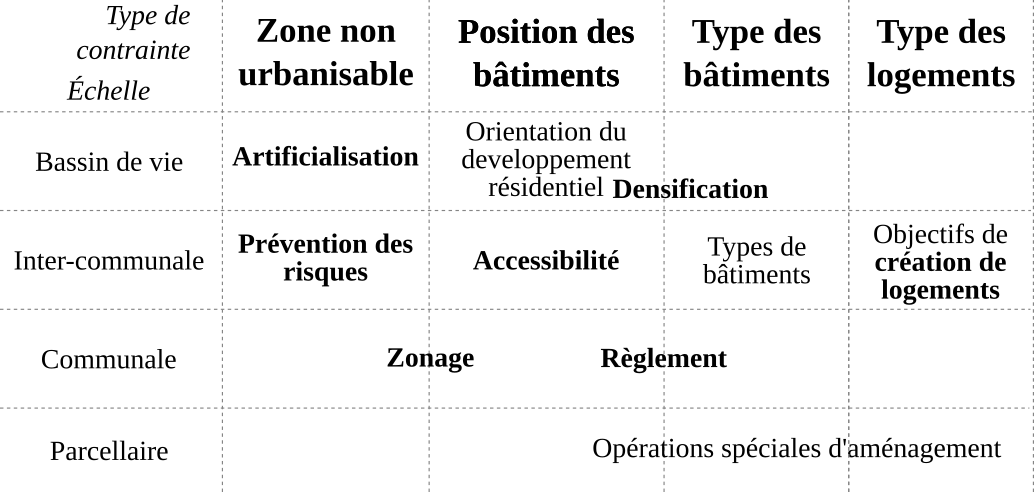
\includegraphics[width=11cm]{Images/synthese-doc.png}	
\end{frame}


%\begin{frame}{Objectifs principaux}
%	\begin{itemize}
%		\item Étude des effets des documents d'aménagement sur le développement résidentiel
%		\item Développer un outils pour permettre aux rédacteurs de les rendre plus efficaces
%	\end{itemize}
%\end{frame}

\begin{frame}{Enjeux : concordance des documents d'urbanisme}
	\begin{itemize}
		\item Différentes \textbf{échelles} d'application
		\item Différents \textbf{rédacteurs}
		\item Objectifs divers
		\item Effets potentiellement \textbf{contradictoires}
	\end{itemize}
	\uncover<2->{	
		\begin{block}{}
			\textbf{Anticiper} les effets des documents d'urbanisme en les \textbf{simulant} afin d'améliorer leurs \textbf{concordance} %et d'expliciter leurs \textbf{}
		\end{block}
	}
\end{frame}

\begin{frame}{Moyens : Outils d'aide à la décision pour l'aménagement}
\centering
		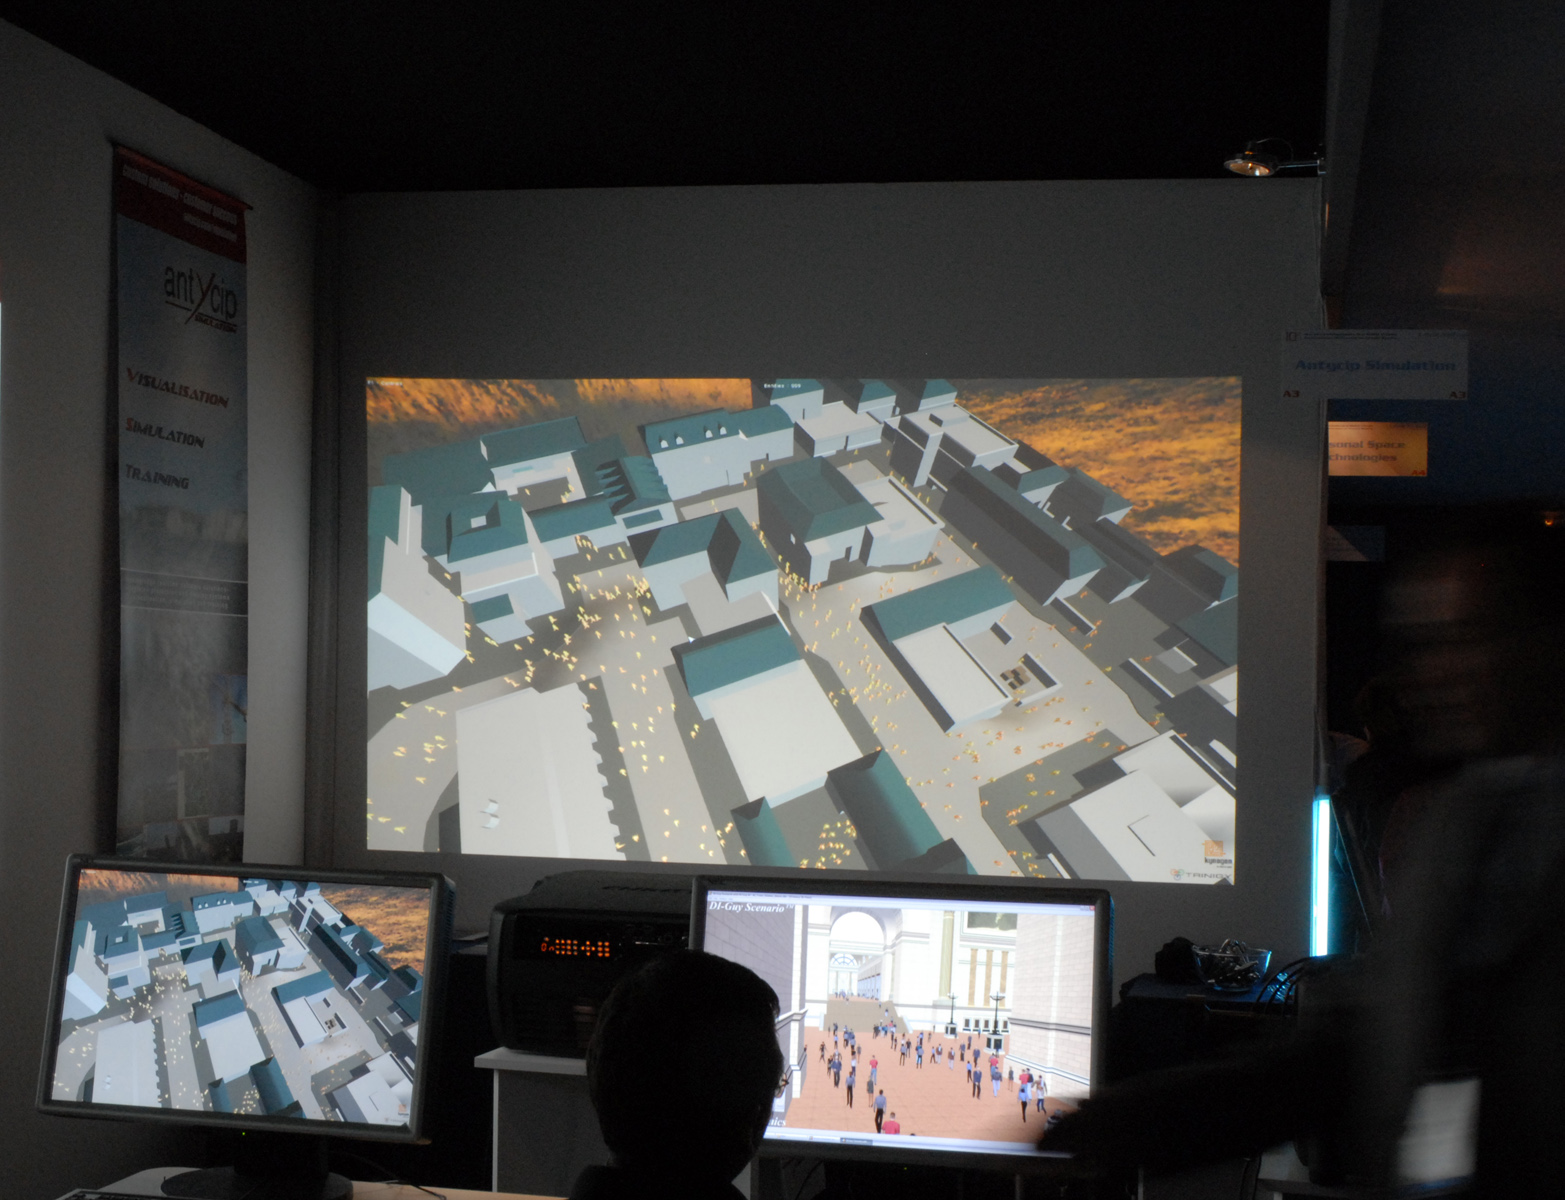
\includegraphics[width=5.7cm]{Images/bureau.jpg}	
\\
		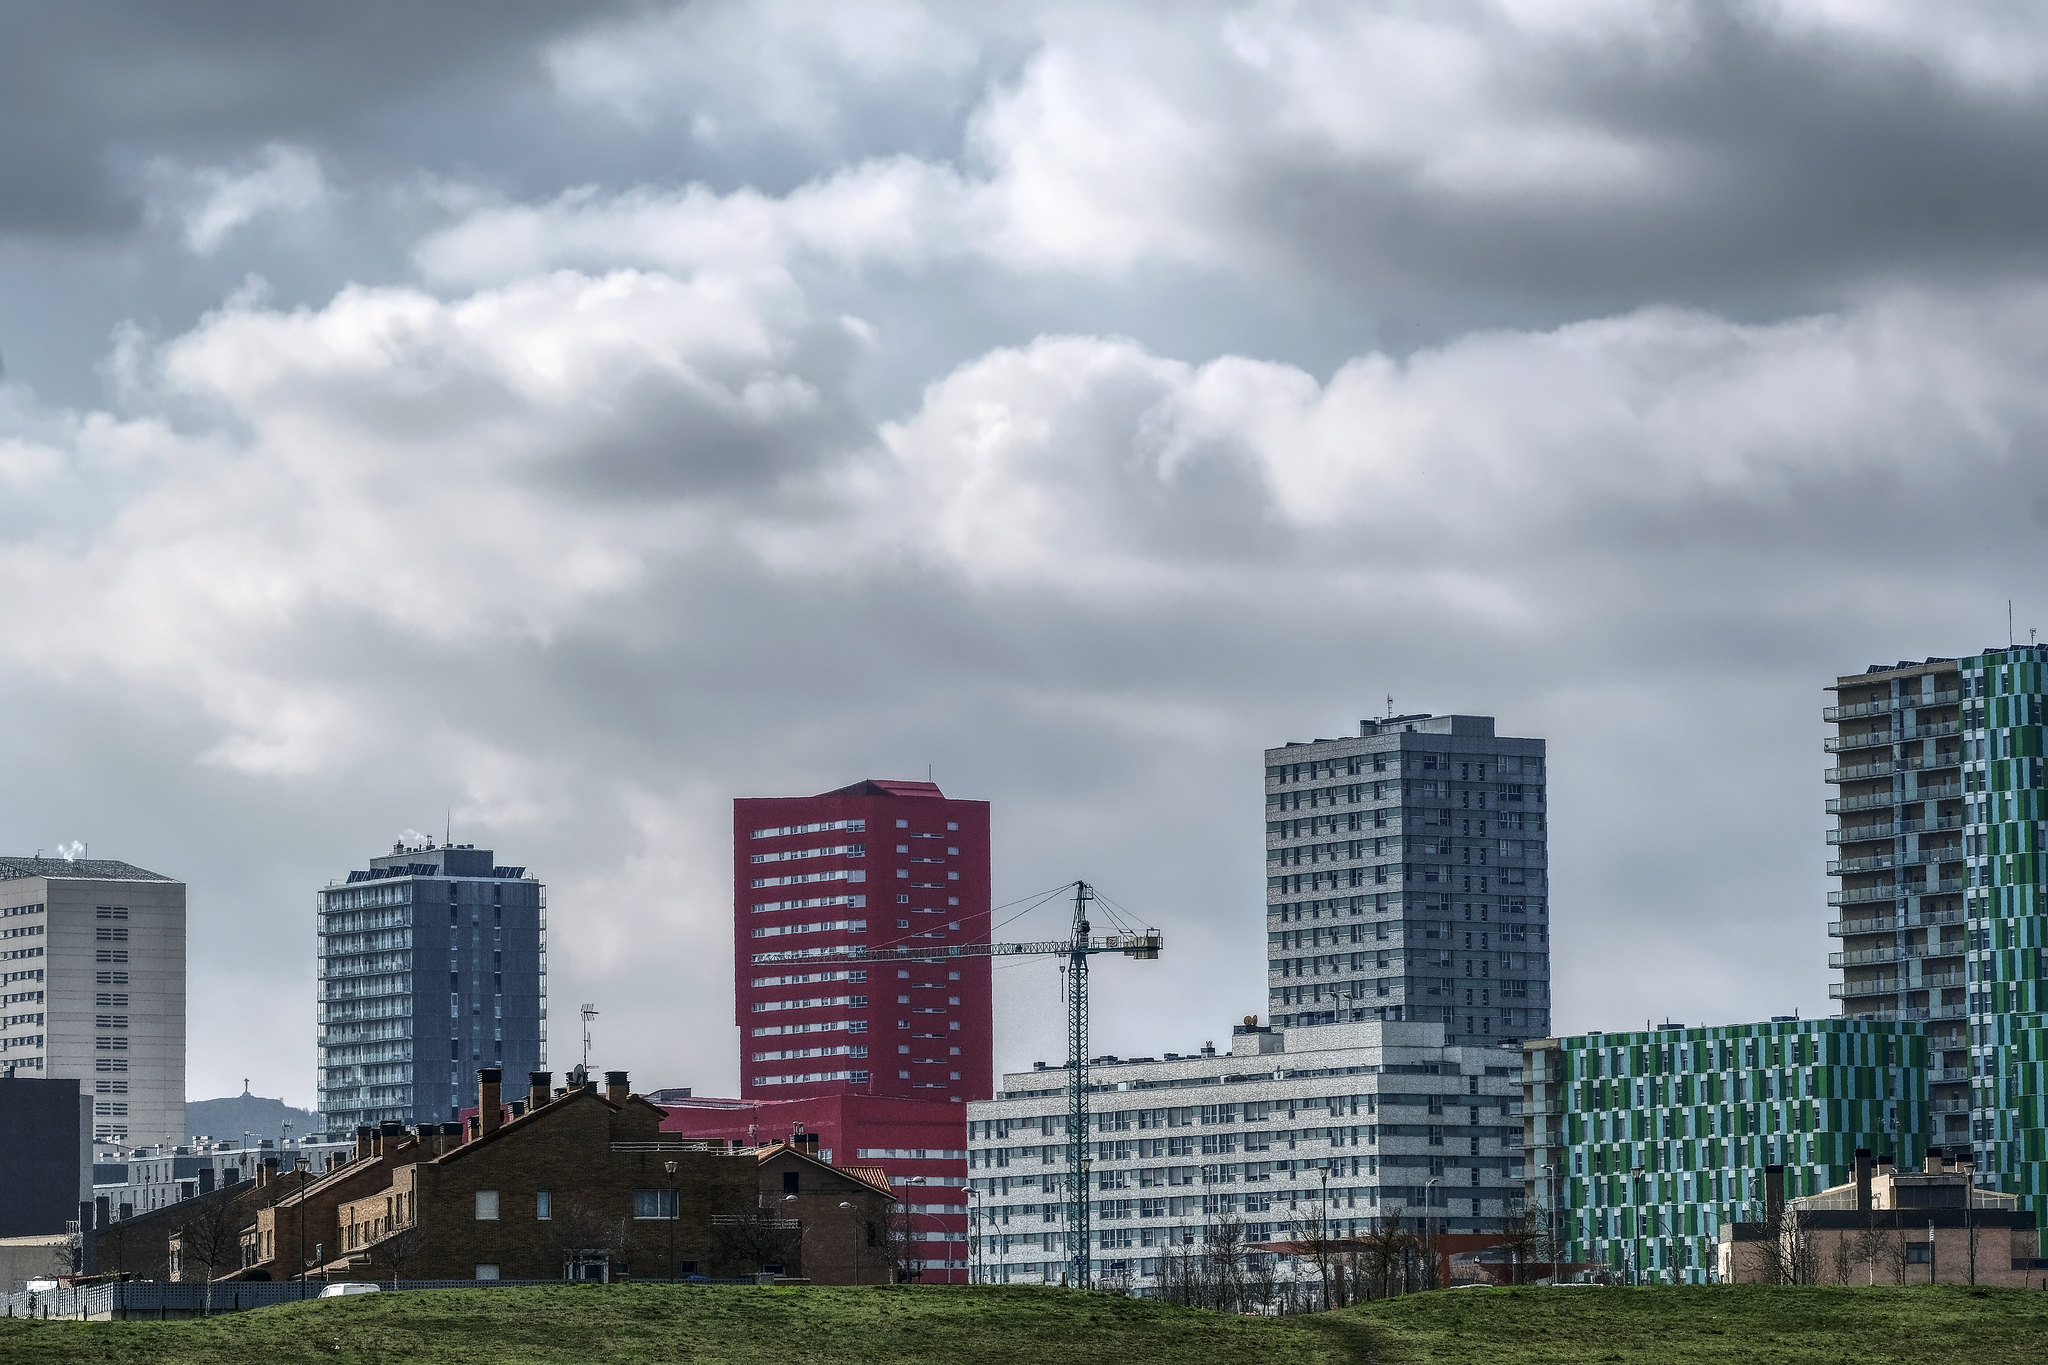
\includegraphics[width=5.7cm]{Images/simcity.jpg}	
\end{frame}

\begin{frame}{Moyens : Outils d'aide à la décision pour l'aménagement à visée prospective}
\begin{block}{}
	\textbf{Objectifs}\\
	Modélise \textbf{un ou plusieurs phénomènes} réels\\
	Simule les \textbf{évolution} probables du système étudié\\
%	Simulations réapplicables et systématisables\\
\end{block}
\uncover<2->{	
	\begin{block}{}
		\textbf{Utilisations}\\
		Représenter des futurs potentiels, recherchés, redoutés\\
		Permettre de comparer plusieurs \textbf{scénarios}	
	\end{block}
}
\uncover<3->{	
	\begin{block}{}
		\textbf{Limites}\\
		Approximations inhérentes aux \textbf{niveaux de détails} et à la \textbf{modélisation} des phénomènes\\
		Utilisation pour l'aide à la conception de documents %et non pour une rédaction \textit{automatisée}
	\end{block}
}
\end{frame}

\begin{frame}{État de l'art des modèles de simulation du développement résidentiel}
	Différents modèles permettent d'étudier le développement résidentiel :
	\\
	À une échelle régionale, de nombreuses familles de modèles
\end{frame}

\begin{frame}{État de l'art des modèles de simulation du développement résidentiel}
À une échelle locale, d'autre dynamiques
Différents modèles permettent d'étudier le développement résidentiel :
\\
À une échelle régionale, de nombreuses familles de modèles
\end{frame}

\begin{frame}{Détection d'emplacements intéressants à urbaniser}
Faire un tableau avec les avantages et les inconvénients des différentes approches
	\begin{itemize}
		\item LUTI (UrbanSim, MobiSim)
		\item Modèles Multi Agents (Artznete 10)
		\item Aide à la décision multi objective
		\item Analyse du foncier (UrbanSimul)
		\item Automate cellulaire
	\end{itemize}
\end{frame}

\begin{frame}{Recomposition du tissus parcellaire}
	(trouver des références sur l'étude des parcelles cf. rapport JT)
	\begin{itemize}
		\item Algorithmes de découpages parcellaire	existent (Vanegas 12).. 
	\end{itemize}
\end{frame}

\begin{frame}{Simulation des bâtiments}
	\begin{itemize}
		\item Modèle paramétrique (Coors 2009)
		\item Modèle d'optimisation sous contrainte	: \textbf{SimPLU}
	\end{itemize}
\end{frame}

\begin{frame}{Problématique}
\only<1>{Il n'existe pas de modèles permettant de simuler un développement résidentiel multi-échelle, multi-contraint et suffisamment descriptif pour s'adapter aux contraintes locales.}
\only<2>{Comment \textbf{simuler} le \textbf{développement résidentiel} d'une région urbaine à un niveau \textbf{très détaillé}, afin d'\textbf{assister} à la rédaction des différents types de \textbf{documents de planification et d'urbanisme} ?}
\end{frame}

\begin{frame}{Objectifs de la thèse}
		\begin{block}{}
		Création d'un modèle de développement résidentiel afin de simuler des évolutions~:
		\begin{itemize}
			\item réaliste (respectant les règlements et les contraintes physiques et fonctionnelles)
			\item multi-échelle (d'une agglomération à la parcelle)
			\item ouvert (réutilisable et discutable) %\textit{Préciser les objectifs (back/forecasting)} ? ou avant? 
		\end{itemize}
	\end{block}
	Couplage de modèles pré-existant~: \textbf{ArtiScales} 
\end{frame}




%\section[Plan]{Plan de la présentation}




\begin{frame}{Plan de la présentation}
	\begin{itemize}
		\item Présentation d'\textbf{ArtiScales}
		\item Présentation des \textbf{modules} d'ArtiScales
		\item Présentation d'une \textbf{expérimentation} d'ArtiScales
	\end{itemize}
\end{frame}




\section{ArtiScales}





\begin{frame}{Contraintes à modéliser}
	\only<1>{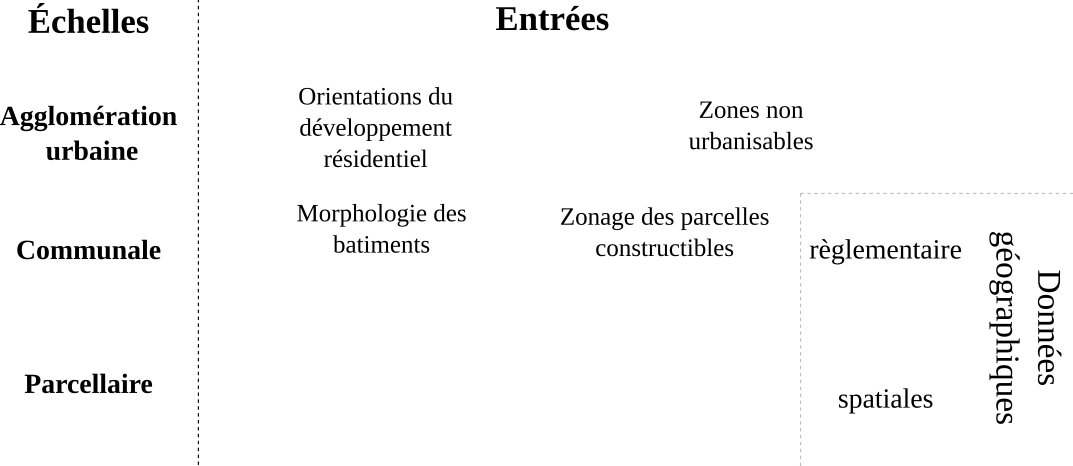
\includegraphics[width=10.7cm]{Images/contraintes0.png}}
	\only<2>{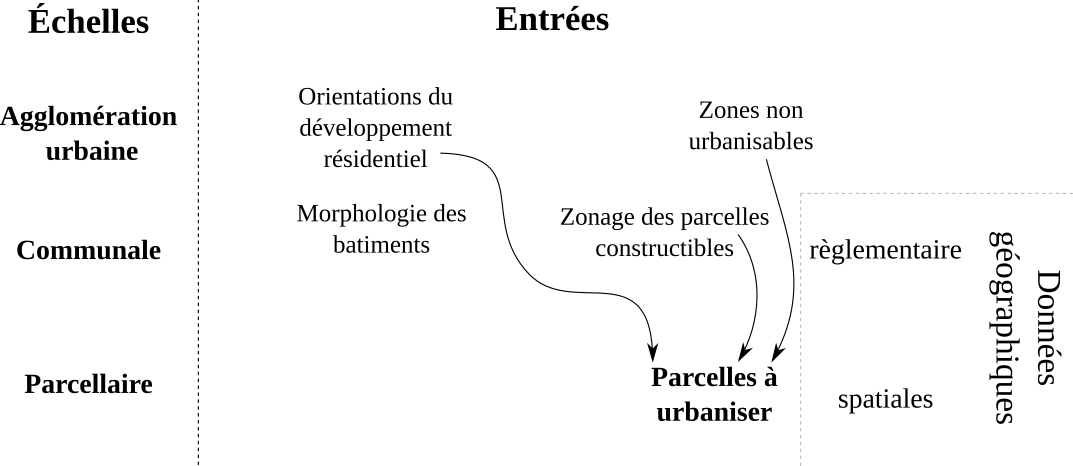
\includegraphics[width=10.7cm]{Images/contraintes1.png}}
	\only<3>{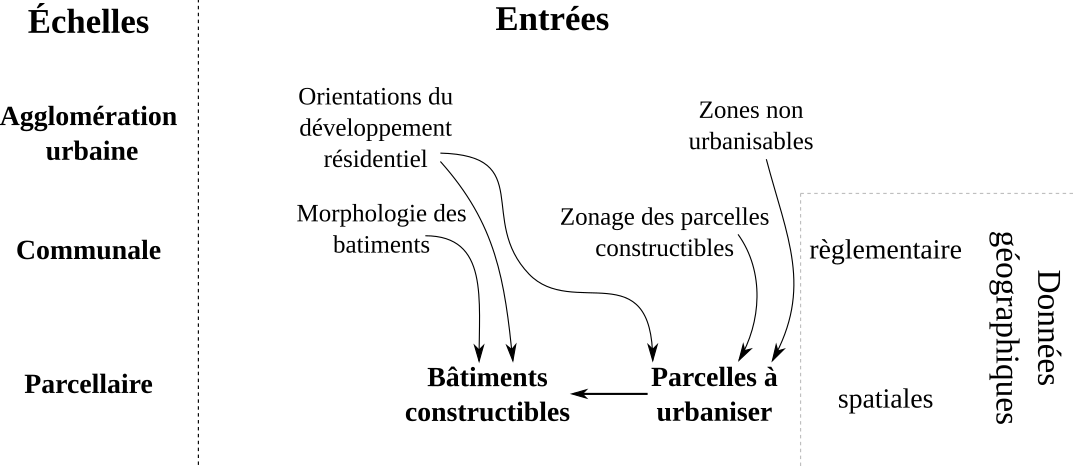
\includegraphics[width=10.7cm]{Images/contraintes2.png}}
	\only<4>{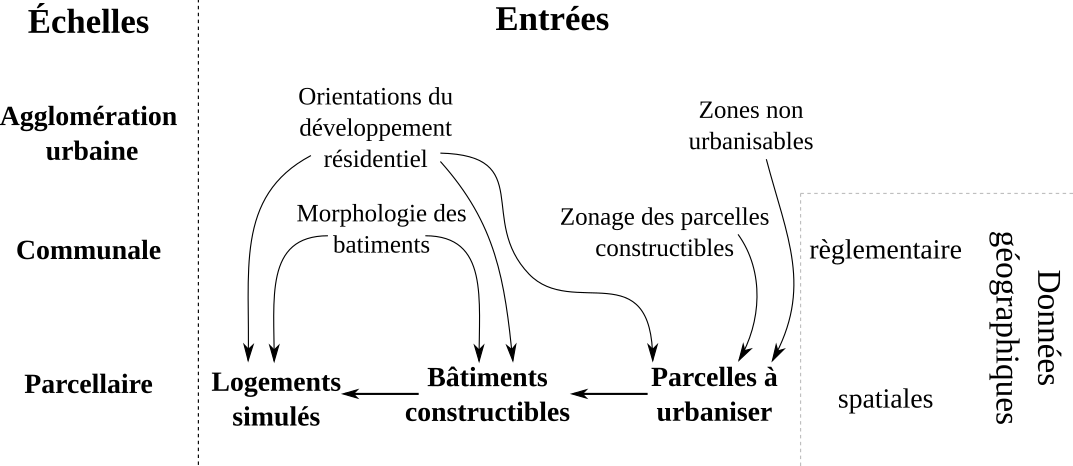
\includegraphics[width=10.7cm]{Images/contraintes3.png}}
\end{frame}

\begin{frame}{Résultats nécessaires au modèle}
		\begin{itemize}
			\item Estimation de logements de différents types
			\item Bâtiments en trois dimensions
			\item Modification parcellaire
			\item Densité de logements et de bâtiments
			\item 
		\end{itemize}
\end{frame}

\begin{frame}{Entrées nécessaires au modèle}
	\begin{block}{}
		\begin{itemize}
			\item Morphologie des bâtiments (réelle et réglementaire)
			\item Parcelles et zonages
			\item Orientations et contraintes sur la forme du développement résidentiel
		\end{itemize}
	\end{block}
	\uncover<2->{
		\begin{block}{}
			Couplage de modèles de simulation~: \textbf{ArtiScales} 
		\end{block}
	}
\end{frame}

\begin{frame}{ArtiScales}
	Trois différents modèles nécessaire~:
	\begin{itemize}
		\item Détection d'emplacements intéressants à urbaniser au sein de l'agglomération
		\item Recomposition du tissus parcellaire
		\item Simulation sous contraintes des bâtiments
	\end{itemize}
\end{frame}



\begin{frame}{ArtiScales : Couplage de modèles}
	\centering
	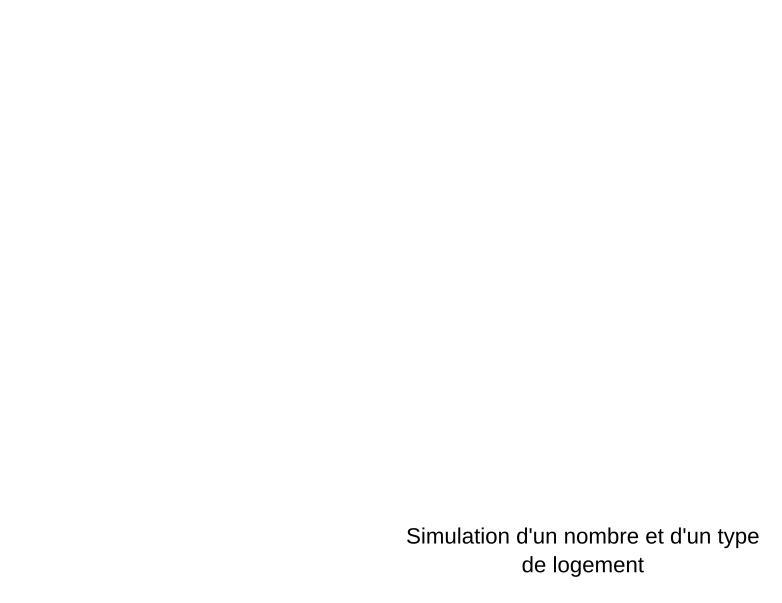
\includegraphics[width=8cm]{Images/schemGenPrez0.png}
\end{frame}


\begin{frame}{ArtiScales : Travaux entrepris}
	\centering
	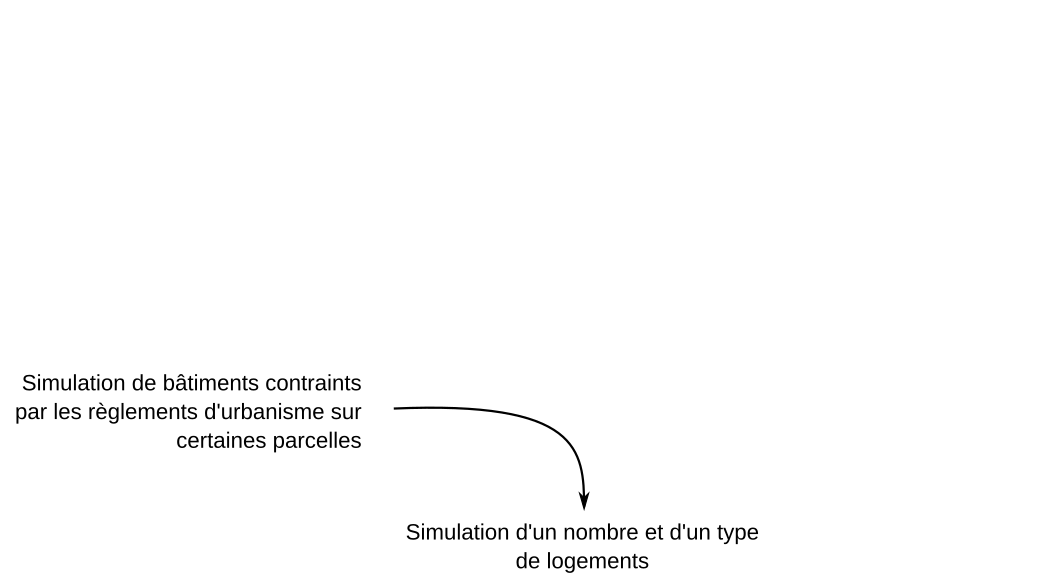
\includegraphics[width=8cm]{Images/schemGenPrez1.png}
\end{frame}


\section[MUP-City]{MUP-City et le développement résidentiel régional}


\begin{frame}{MUP-City}
	\centering{
\includegraphics[width=3cm]{Images/mup.png}}
	\\
	Simulation multi-échelle du développement résidentiel 
	\begin{itemize}
		\item Considère une \textbf{région urbaine} entière
		\item Propose une \textbf{organisation spatiale locale}
		\item Met en œuvre différentes \textbf{orientations d'aménagement}
	\end{itemize}
	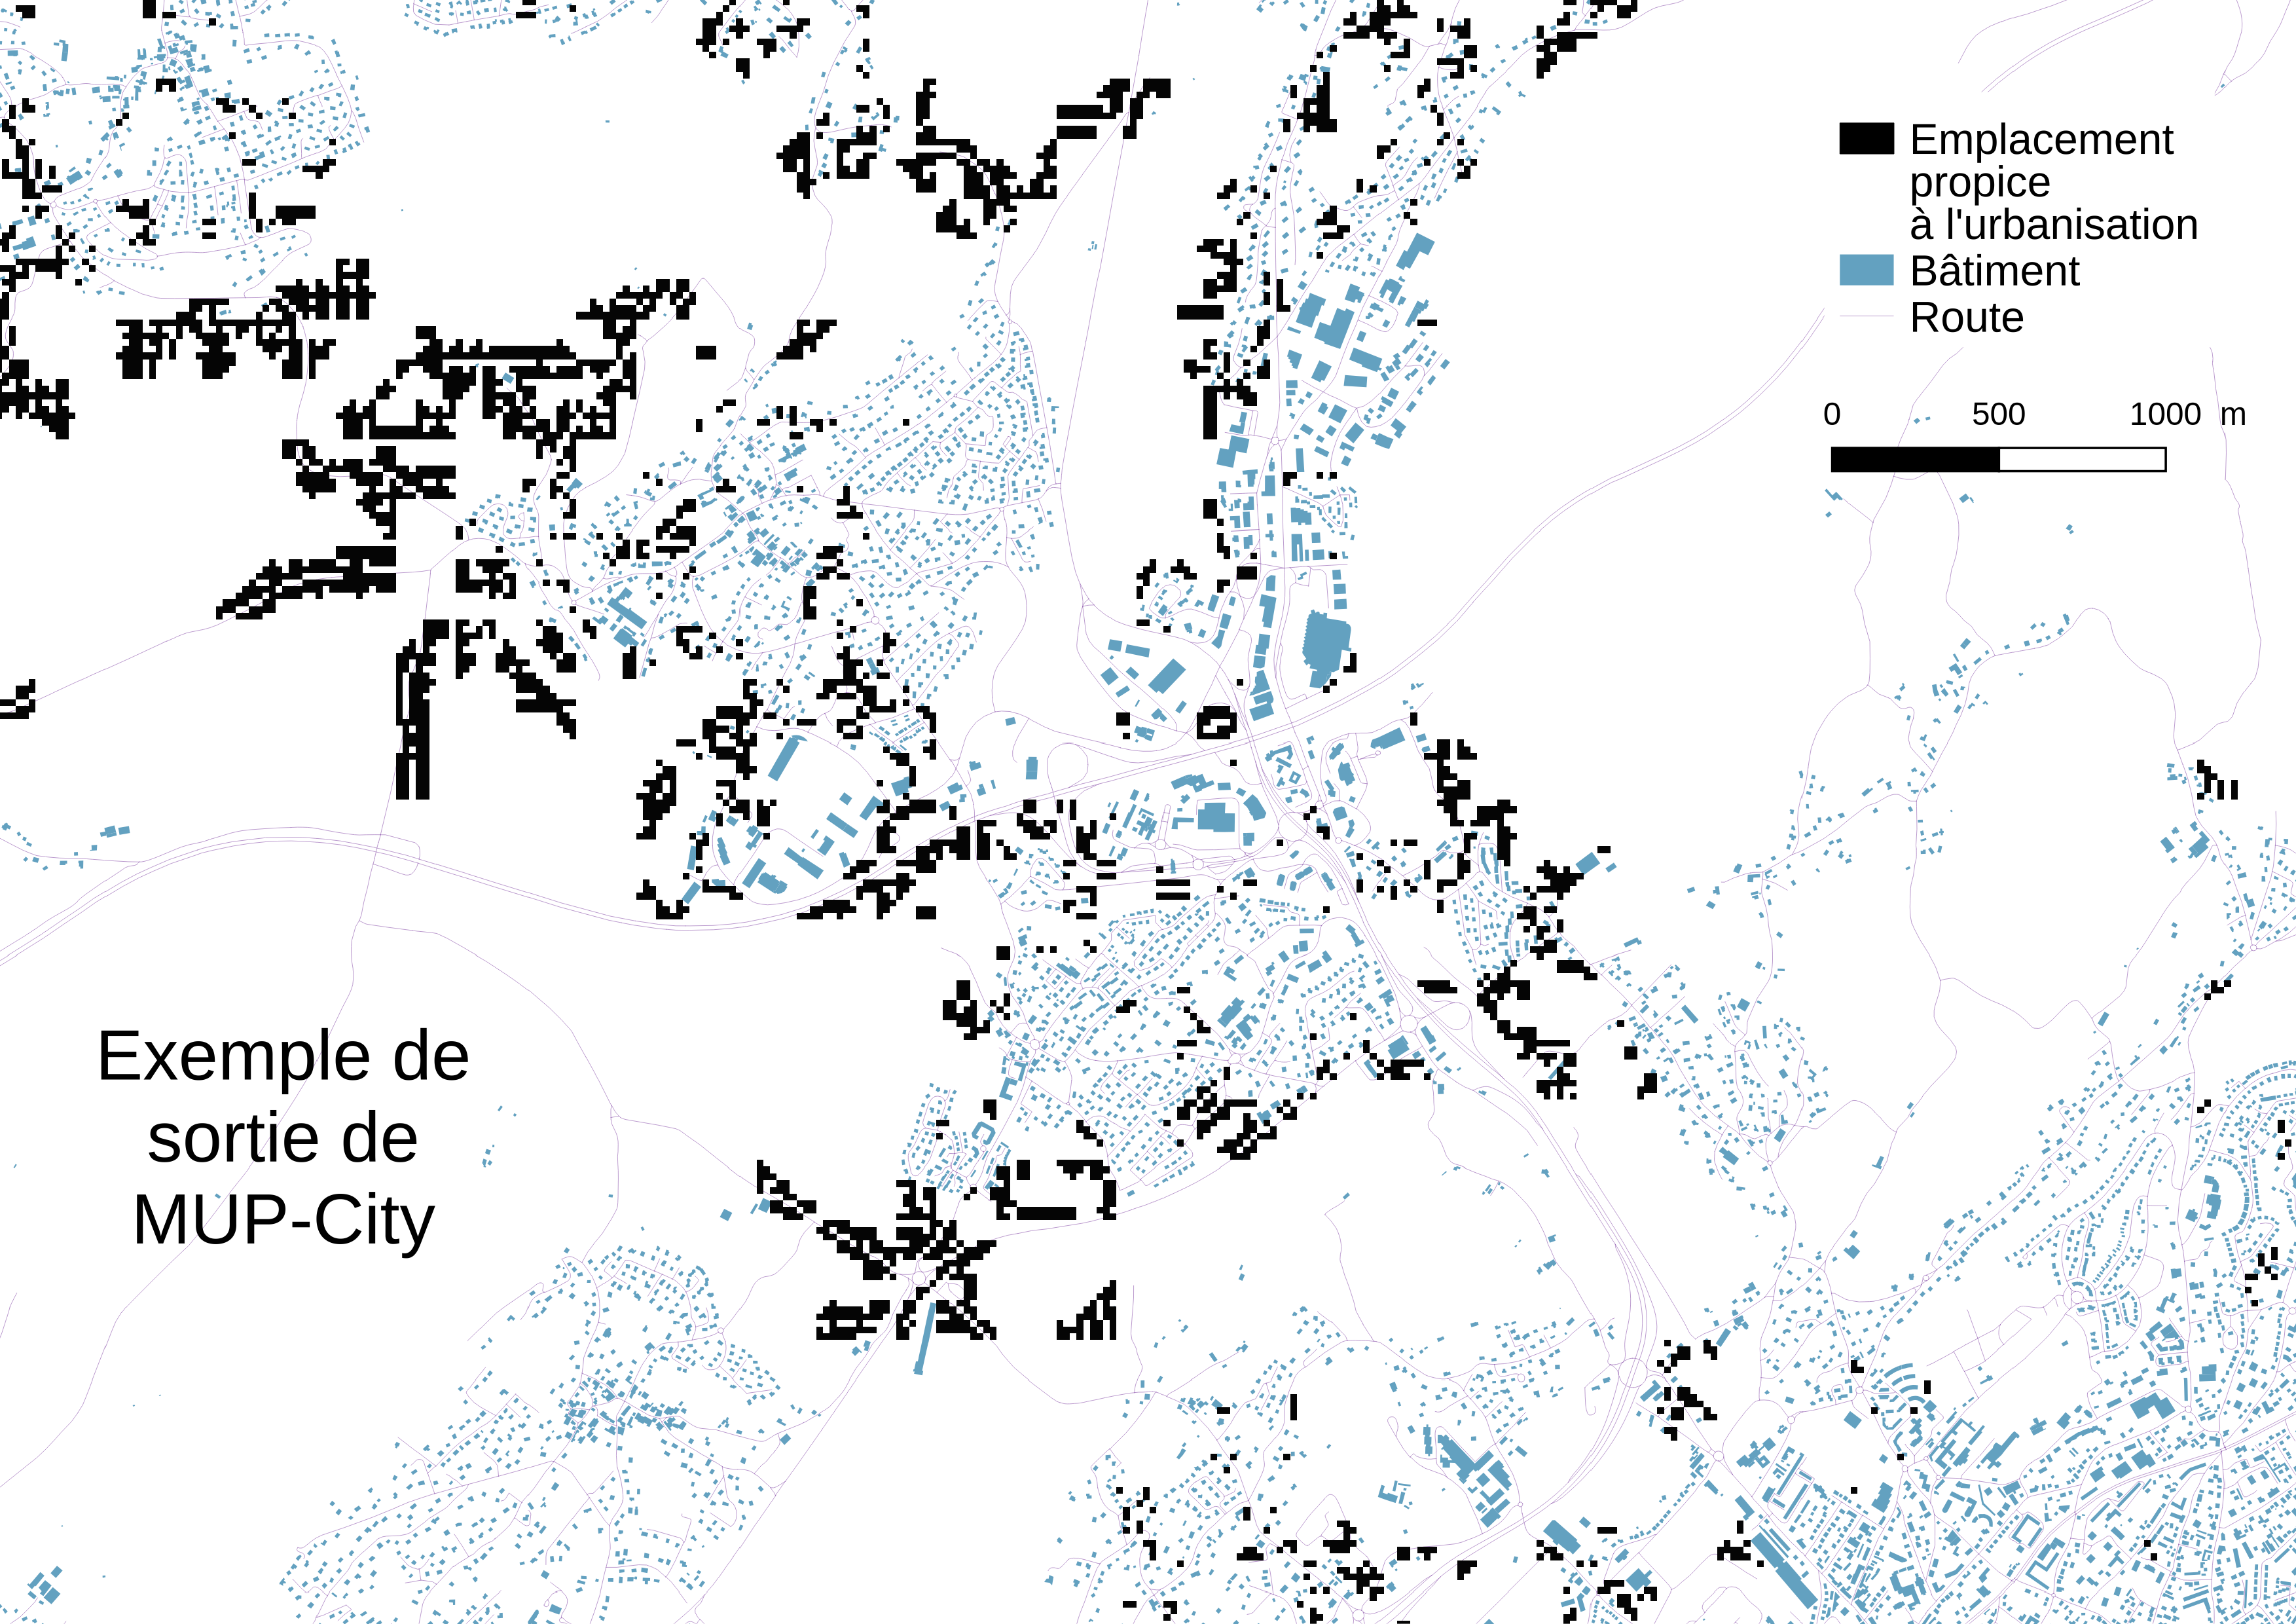
\includegraphics[width=6.5cm]{Images/ex-sorties-mup.png}
\end{frame}

\begin{frame}{MUP-City: entrées et sorties}
	\textbf{Entrées}
	\begin{itemize}
		\item Environnement vectoriel 
		\item Paramètres de simulation et d'orientations d'aménagements
	\end{itemize}
	\textbf{Sorties}
	\begin{itemize}
		\item \textbf{Cellules de 20m} représentant des emplacements potentiellement urbanisables
		\item Évaluations suivant des critères morphologiques et d'accessibilité
	\end{itemize}
	\begin{block}{}\centering{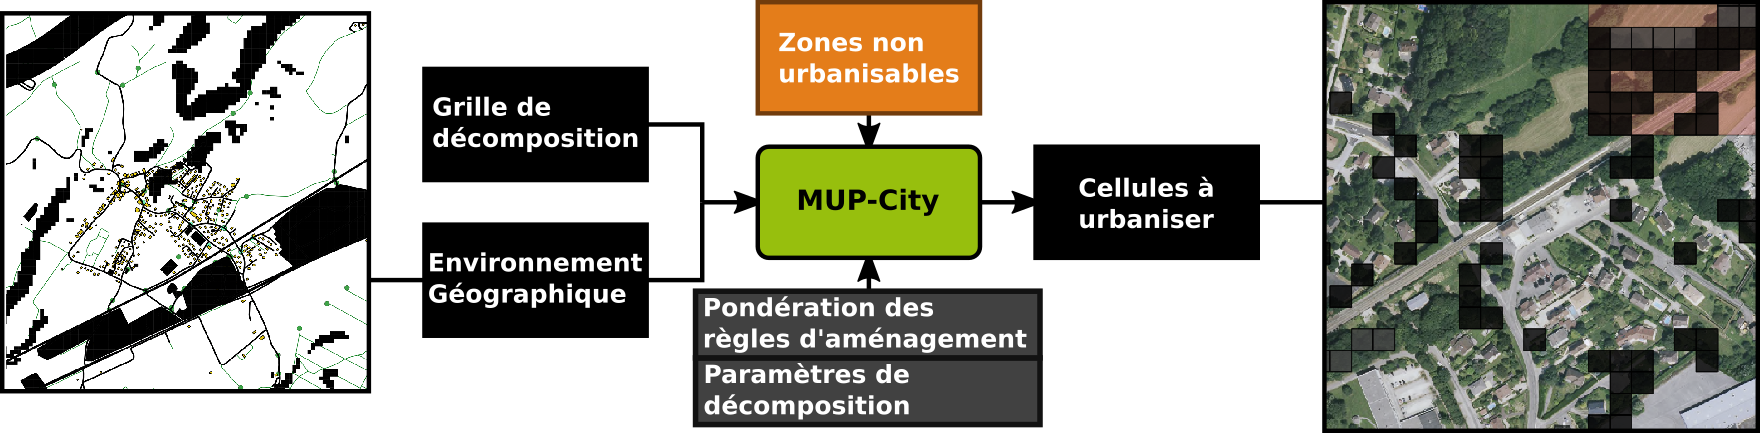
\includegraphics[width=9.5cm]{Images/schema_mupcity.png}}\end{block}
\end{frame}

\begin{frame}{MUP-City: analyse de variabilité}
	\begin{block}{Principe}
				Analyser la variation des résultats de simulation d'un modèle\\
				Sélection de \textbf{configurations résidentielles} à exploiter
			\end{block}

	\begin{block}{Objectifs}
				\textbf{Fiabilité} des résultats de simulation\\
				Sélection de \textbf{configurations résidentielles} à exploiter
			\end{block}

	\begin{block}{Verrous}
				Définition des indicateurs utilisés pour caractériser les résultats\\
			\end{block}
	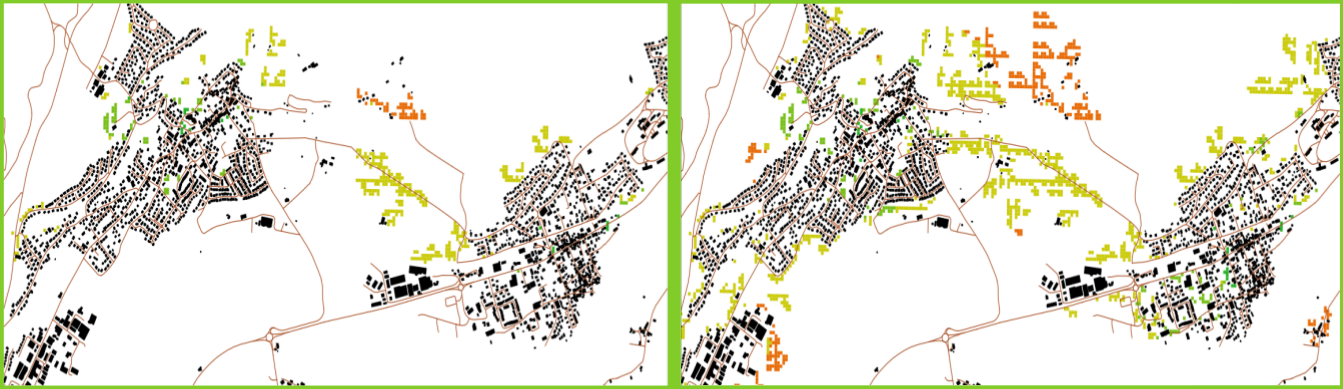
\includegraphics[width=11cm]{Images/ex-sorties-mup2.png}
\end{frame}

\begin{frame}{MUP-City: analyse de variabilité - Grille d'analyse proposée}
	\begin{block}{Trois types de variation des paramètres}
		Étude du caractère aléatoire du modèle : \alert{Stabilité}\\
		Étude des paramètres dits \alert{techniques}\\
		Étude des paramètres dits \alert{scénaristiques}
	\end{block}
\end{frame}

\begin{frame}{Exemples}
	une variation pour chaque type ? 
\end{frame}

\section[Parcel Manager]{Parcel Manager pour la gestion du tissus parcellaire}

\begin{frame}{Présentation du modèle}
 	\centering{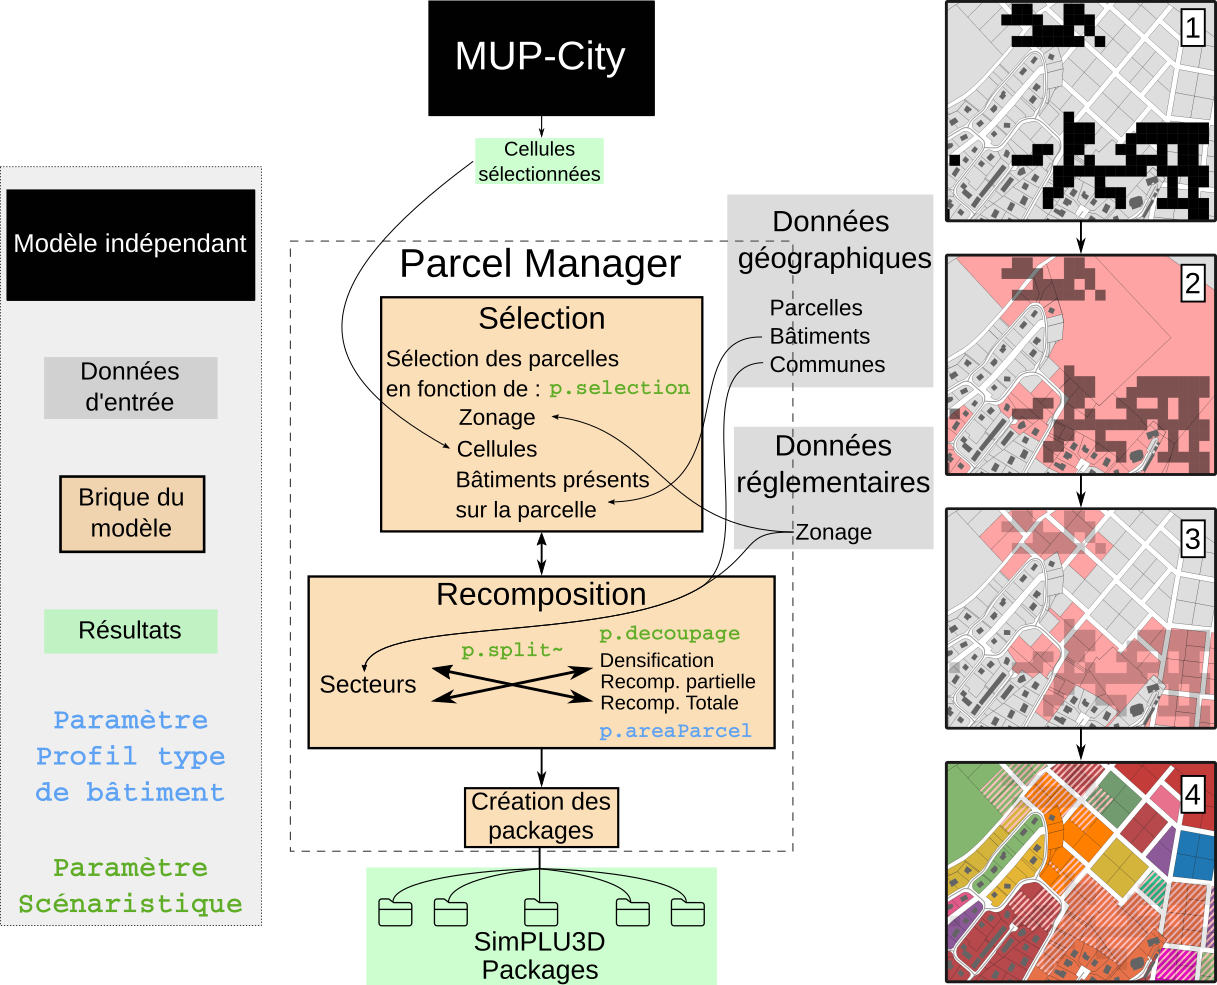
\includegraphics[width=9cm]{Images/schemGenParcelManager.png}}
\end{frame}

\begin{frame}{Trois types de décompositions parcellaires}
	
\end{frame}



\section[SimPLU]{SimPLU et la simulation de bâtiments}



\begin{frame}{Présentation de SimPLU}
	\centering{\textbf{SimPLU}}
	\\
	Génère des configurations bâties en 3D
	\begin{itemize}
		\item Produit un ensemble de configurations potentiellement constructibles selon les \textbf{contraintes du PLU}
		\item Optimise certains paramètres afin de poursuivre différents \textbf{objectifs de construction}
		\item Simule le comportement d'agents constructeurs
	\end{itemize} 
	\centering{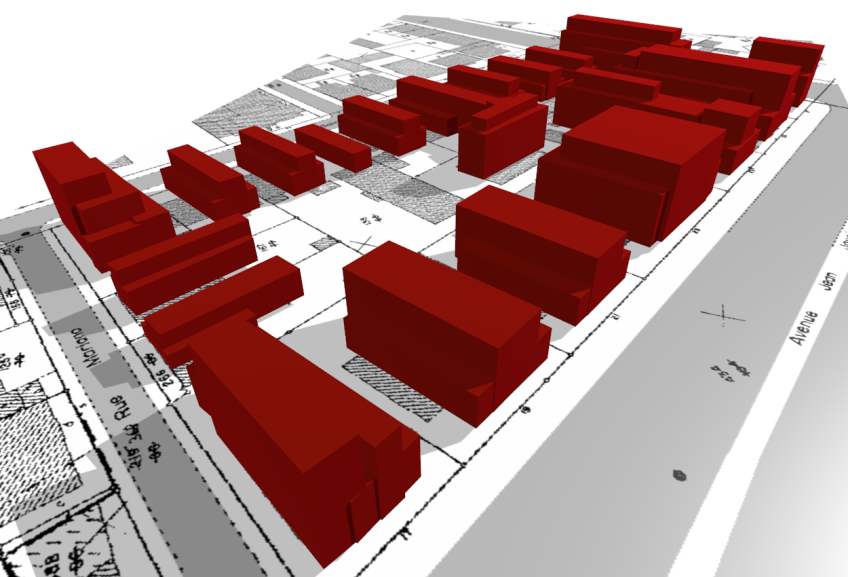
\includegraphics[width=5cm]{Images/SimpluOutput.png}}
\end{frame}

\begin{frame}{SimPLU: entrées et sorties}
	\begin{block}{Entrées}

		\begin{itemize}
			\small
			\item Parcelle au sein d'un îlot urbain
			\item Contraintes paramétriques sur les ``boîtes'' pour simuler un type de bâtiment prédéfini
			\item Fonction d'optimisation
		\end{itemize}
		\textbf{Sortie}
		\begin{itemize}
			\small
			\item Configuration en 3D représentant un potentiel constructible
		\end{itemize}
	\end{block}
	\begin{block}
		\centering{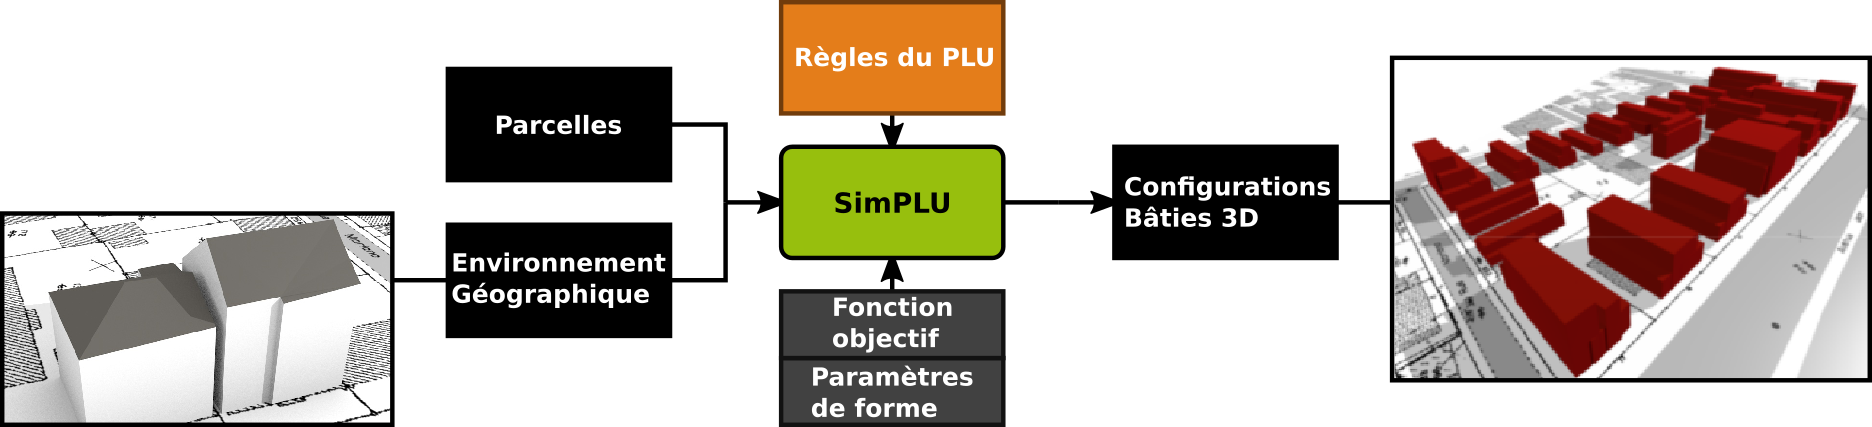
\includegraphics[width=11cm]{Images/schema_simplu.png}}
	\end{block}		
\end{frame}

\begin{frame}{Contraintes paramétriques sur les ``boîtes''}
		\begin{block}{}
			Cinq types de bâtiments~:\\
		\end{block}
	
	\only<1>{\textbf{Maison isolée}\\
		\begin{block}{}
		\centering{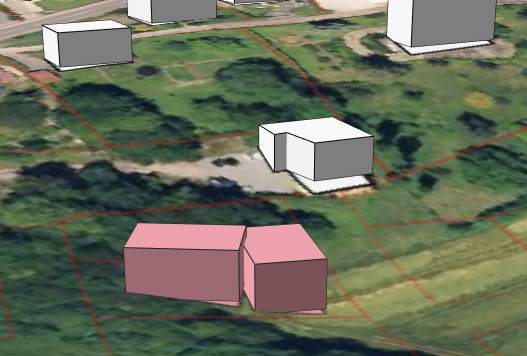
\includegraphics[width=7cm]{Images/detachedHouse.png}}	
		\end{block}
	}
	\only<2>{\textbf{Pavillon de lotissement}\\
		\begin{block}{}
		\centering{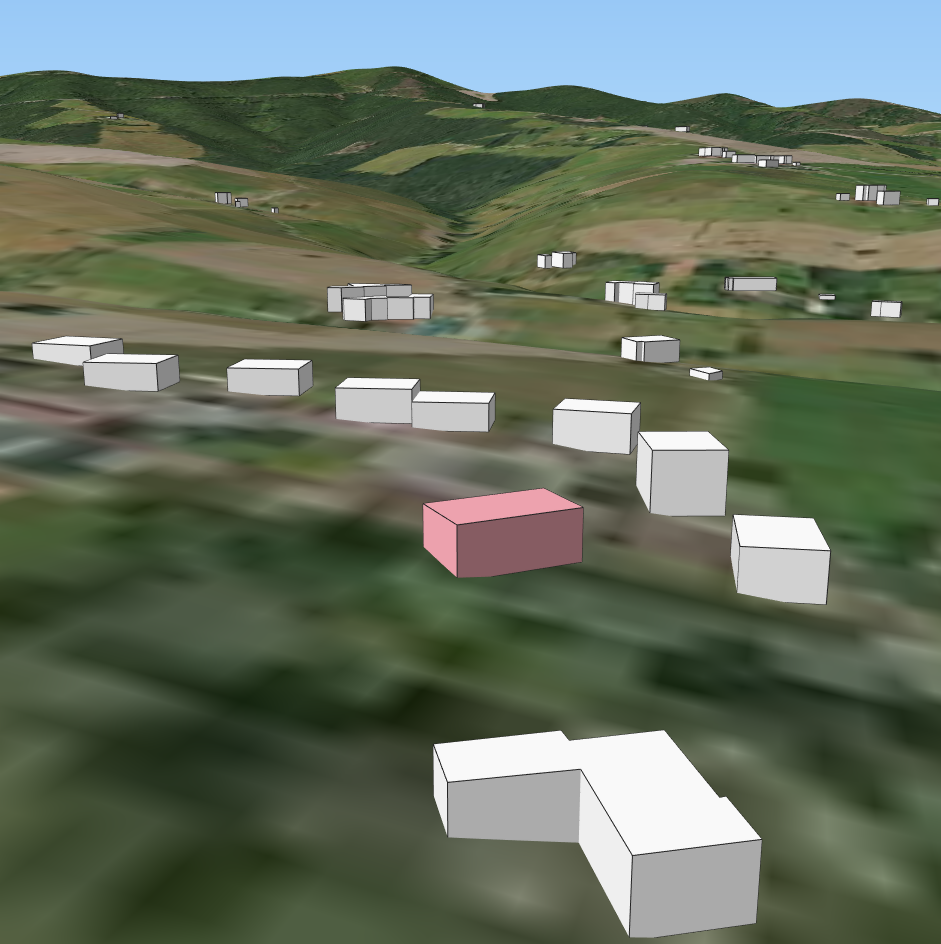
\includegraphics[width=5cm]{Images/smallBlock.png}}	
		\end{block}
	}
	\only<3>{\textbf{Immeuble d'habitat intermédiaire}
		\begin{block}{}
		\centering{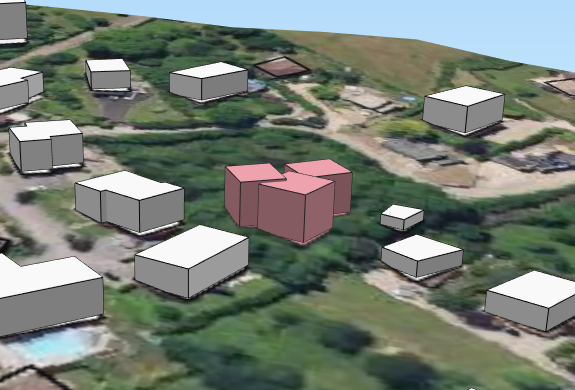
\includegraphics[width=7cm]{Images/multiFamilyHouse.png}}	
		\end{block}
	}
	\only<4>{\textbf{Petit immeuble collectif}\\
		\begin{block}{}
		\centering{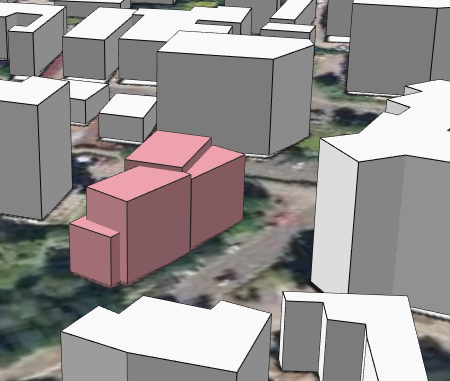
\includegraphics[width=7cm]{Images/smallBlockFlat.png}}	
		\end{block}
	}
	\only<5>{\textbf{Immeuble collectif de taille moyenne}\\
		\begin{block}{}
		\centering{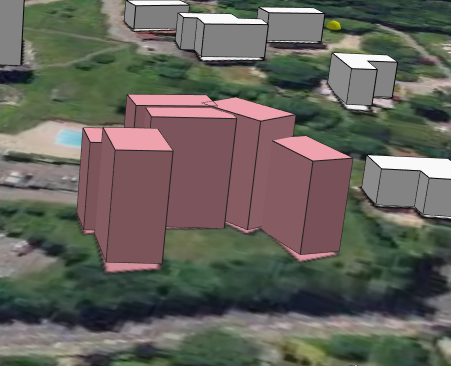
\includegraphics[width=7cm]{Images/midBlockFlat.png}}	
		\end{block}
	}
\end{frame}

\begin{frame}{Contrainte d'optimisation des bâtiments}
	\begin{block}{}
		\centering
		\textbf{Optimisation du volume des bâtiments}
	\end{block}
	\centering{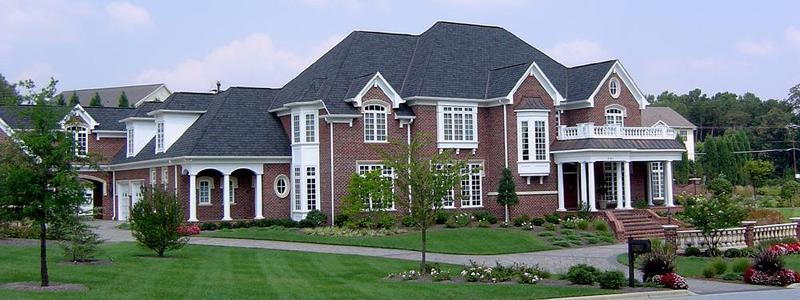
\includegraphics[width=11cm]{Images/fatAmericanHouse.jpg}}
\end{frame}

\begin{frame}{SimPLU: étude des sorties - Exemple}
	\begin{block}{}
		Étude du caractère aléatoire : très faible \textit{(Brasebin, 2014)}
	\end{block}
	\begin{block}{}
		Étude de l'effet des paramètres techniques~: potentiellement important \textit{(soulevé par l'expérimentation de la thèse)}
	\end{block}
	\begin{block}{}
		Étude de l'effet des paramètres scénaristiques~: \textit{(Chapron, Brasebin, Perret et al, 2017)}
		
\end{block}
	\centering{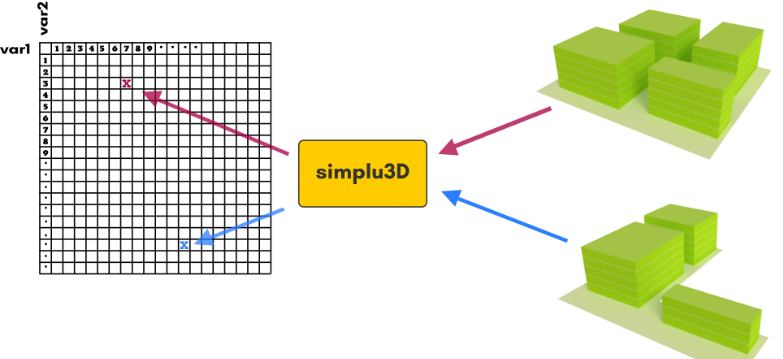
\includegraphics[width=7cm]{Images/simpluOutputSpace.png}}\\
	\FontPetit\centering{\textit{ }}
\end{frame}

\note{Explorations systématiques visant à la mise au point de de bonnes pratiques pour la création de PLU}



\section[Expérimentation]{Expérimentation d'ArtiScales sur l'agglomération du Grand Besançon}




\begin{frame}{Expérimentation menée au cours de la thèse}
	\begin{block}
		\textbf{Objectifs de l'expérimentation}\\
		\begin{itemize}
			\item Évaluer le fonctionnement d'ArtiScales
			\item Analyser les effets de la variabilité des simulation de MUP-City sur les résultats finaux 
		\end{itemize}
	\end{block}
	\uncover<2->{
		\begin{block}{}
			Application à la Communauté d'Agglomération du Grand Besançon (CAGB)\\
			\vspace{0.1cm}
				\centering{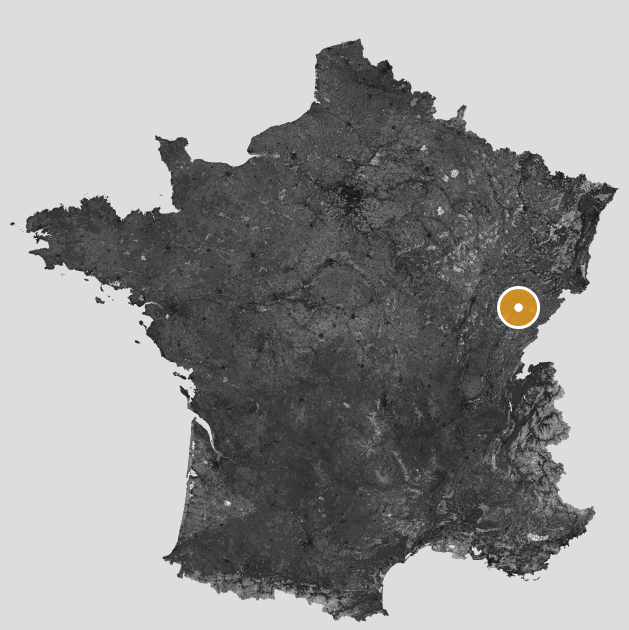
\includegraphics[width=3cm]{Images/france.png}}\\
		\end{block}
	}
\end{frame}

\begin{frame}{Protocole des simulations}
\begin{block}{Deux paramétrage de Parcel Manager et SimPLU3D}
	\begin{itemize}
		\item Forte augmentation de la densité
		\item Augmentation modérée de la densité
	\end{itemize}
\end{block}
\end{frame}

\begin{frame}{Protocole des simulations}
\begin{block}{Deux scénarios de développement résidentiels}
	\begin{itemize}
		\item Densité fractale moyenne et permissif quand aux critères d'évaluation (\textit{Scenario c})
		\item Forte densité fractale et sévère sur les critères d'évaluation (\textit{Scenario d})
	\end{itemize}
\end{block}
\begin{block}{Neuf variantes de développement résidentiels}
\vspace{0.1cm}
	Deux réplications de la modification des paramètres techniques~:
	\begin{itemize}
		\item graine aléatoire
		\item taille des cellules
		\item petits mouvements de la grille de décomposition
		\item grands mouvements de la grille de décomposition
	\end{itemize}
\end{block}
\end{frame}

\begin{frame}{Exécution du code informatique}
	\begin{itemize}
		\item temps théorique sur un ordinateur personnel pour le plan d'expérience~: 285 jours
		\item temps théorique sur la grille de calcul européenne pour le plan d'expérience~: 110 heures
		\item temps constaté sur la grille européenne pour une simulation~: 35 heures
	\end{itemize}
\end{frame}

\subsection{Comparaison des scénarios}

\begin{frame}{Présentation des résultats de simulation}
	\textbf{résolution observé préférentielle : l'armature des communes (peu présent dans le document, mais permet la comparaison avec l'éval du SCoT)}
	présenter l'éval du SCoT
	\\
	Dans une logique décroissante~: (pas forcé de l'indiquer)
	\begin{itemize}
		\item Sélection des parcelles
		\item Simulation de bâtiments
		\item Estimation de logements
		\item Densité de logements 
	\end{itemize}
\end{frame}

\begin{frame}{Sélection parcellaire et consommation foncière}
Chiffres généraux (trouver des comparaisons avec la conso résidentielle d'avant/ de pendant?!)
\\
Comparaison de l'extension/\textit{renouvellement} avec les chiffres du SCoT 
\end{frame}

\begin{frame}{Simulation de bâtiments}
	Types simulés (problèmes dans SimPLU3D)
\end{frame}

\begin{frame}{Simulation de logements}
	Comparaison du nombre de logements simulés avec 
	
	pour tous ou presque: rapport de trois
\end{frame}

\subsection{Comparaison des variantes}

\begin{frame}{Présentation rapide des résultats des variantes}
\textit{pas sur d'en parler si ?}
	\textit{min/max sur les quatre scénarios des tableaux et cartes pour situer ces différences}
\end{frame}


\section{Conclusion}


\begin{frame}{MUP-City : un modèle variable}
	\begin{block}{}
		Plusieurs configurations résidentielles simulés
		\\
		\textbf{conclusions communes sur certaines communes}
	\end{block}
	
	\begin{block}{}
		Possibilité d'utiliser d'autre modèles pour ce bloc? 
	\end{block}
\end{frame}

\begin{frame}{ArtiScales : un modèle hybride}
Mêle des modèles descriptifs à des modèles stylisés~: simulateur hybride
\\
Pas de temporalité - peut être qu'une nouvelle itération devrait être faite tous les 12 ans (cf rapport de 3 x pour chaque 4 ans) pour parvenir à remplir les objectifs ()?
Permettrait aussi de remettre en cause les objectifs (comme dans le cas de Besac, sur-évalués)
		
\end{frame}


\begin{frame}{Utilisation dans l'aide à la décision territoriale}
	Rendre variable certaines restrictions pour voir comment rendre compatible les docs
\\
	par exemple : 
	\begin{itemize}
		\item Zonage (expérimenté dans la thèse)
		\item articles du PLU (hauteur?)
		\item 
	\end{itemize}
\end{frame}

\begin{frame}{Perspectives de recherche : Automatisation des analyses de sensibilité}
	Pour AS : nécessité d'optimisation des simus de SimPLU3D
\end{frame}

\begin{frame}{Perspectives de recherche : Prise en compte de nouveaux processus}
	Nouveaux modes de densification (rendre ArtiScales plus opérant en milieu urbain)
	\\
	Adapter le modèle aux évolutions réglementaires suites aux lois ALUR et ELAN (plus de qualitatif (\textit{performantiel}) grâce à SimPLU3D)
\end{frame}


\begin{frame}[standout]
	\centering
	\begin{block}{}	
		\centering	
		Merci pour votre attention
	\end{block}
	\begin{block}{}
		\centering
		\textit{Everything we do is open source}\\
		\large
		\textbf{MUP-City}: \url{https://sourcesup.renater.fr/mupcity/} \\
		\textbf{SimPLU}: \url{https://github.com/IGNF/simplu3D}\\
		\textbf{PLUCities :} \url{https://github.com/ArtiScales/}  
	\end{block}
\end{frame}

\begin{frame}{Données nécessaire à l'exécution de MUP-City}
	\centering{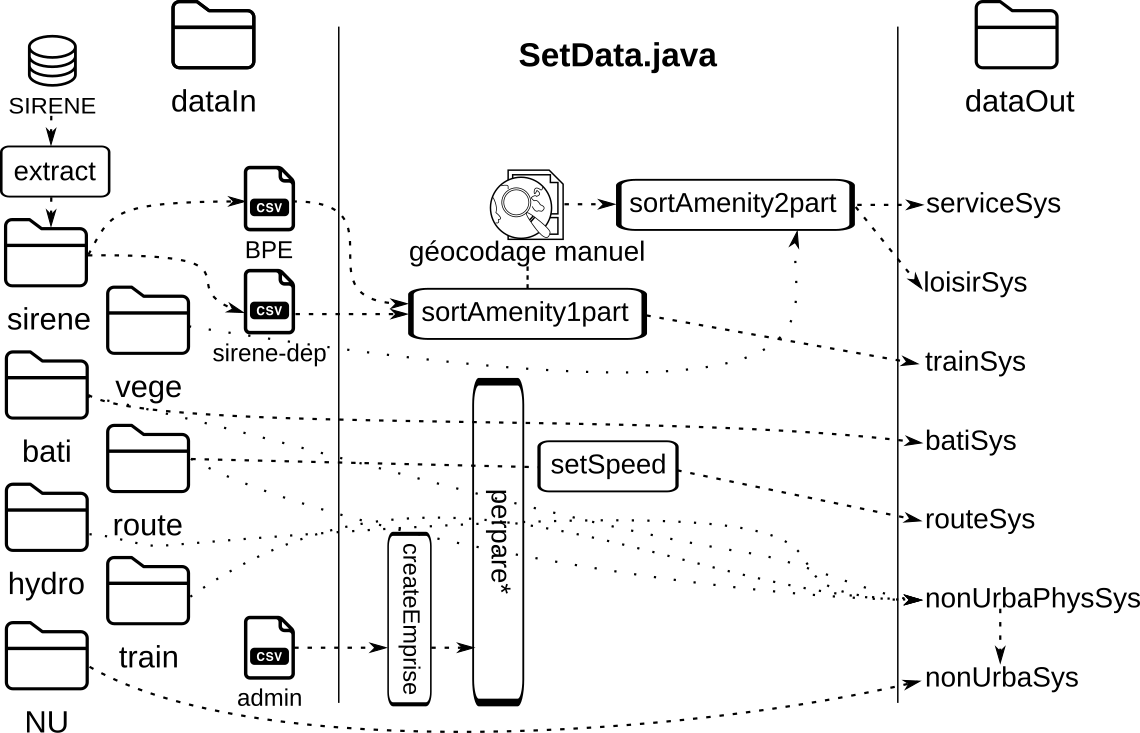
\includegraphics[width=10cm]{Images/schemaSetData.png}}
\end{frame}
\begin{frame}{Données nécessaire à l'exécution de SimPLU}
%		\centering{\includegraphics[width=8.5cm]{Images/simplu3DNbConfigs.png}}
%	\centering{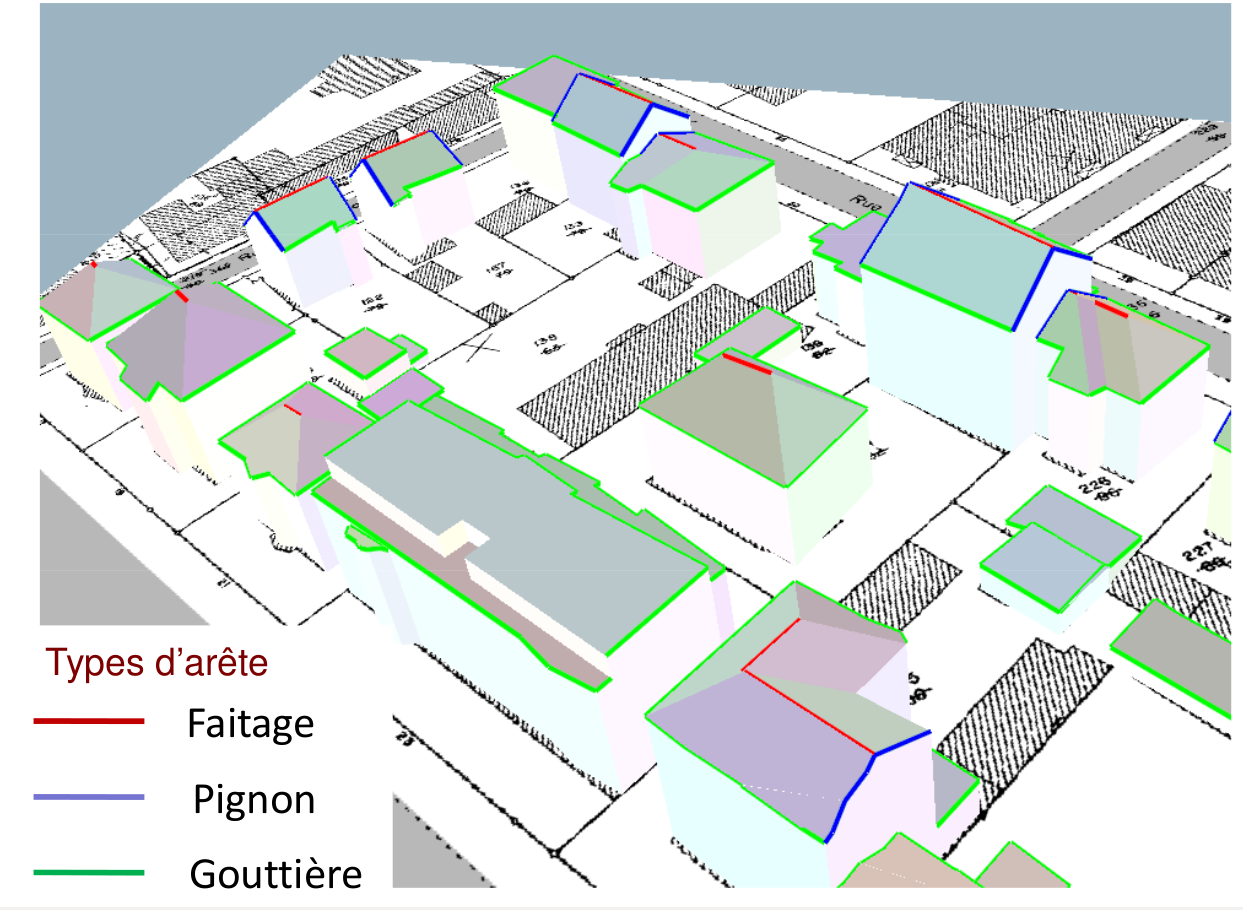
\includegraphics[width=5cm]{Images/simplumodel.png}}
\end{frame}
\end{document}


\begin{frame}{Documents de planification régionale}
Le \textbf{Schéma de Cohérence Territoriale} (SCoT) \textbf{synchronise} les politiques territoriales régionales
\begin{itemize}
	\item Territorialise la construction de logements
	\item Fixe des contraintes morphologiques et de densité
\end{itemize}
\uncover<2->{Le \textbf{Programme Local de l’Habitat} (PLH) fixe la \textbf{politique du logement}
	\begin{itemize}
		\item Précise le nombre et le type de logements prévus par communes
		\item Programme de futures opérations
	\end{itemize}
	\uncover<3>{\textbf{Relation de compatibilité entre ces deux documents}}
}
\end{frame}

\begin{frame}{Documents de planification régionale - Exemple}
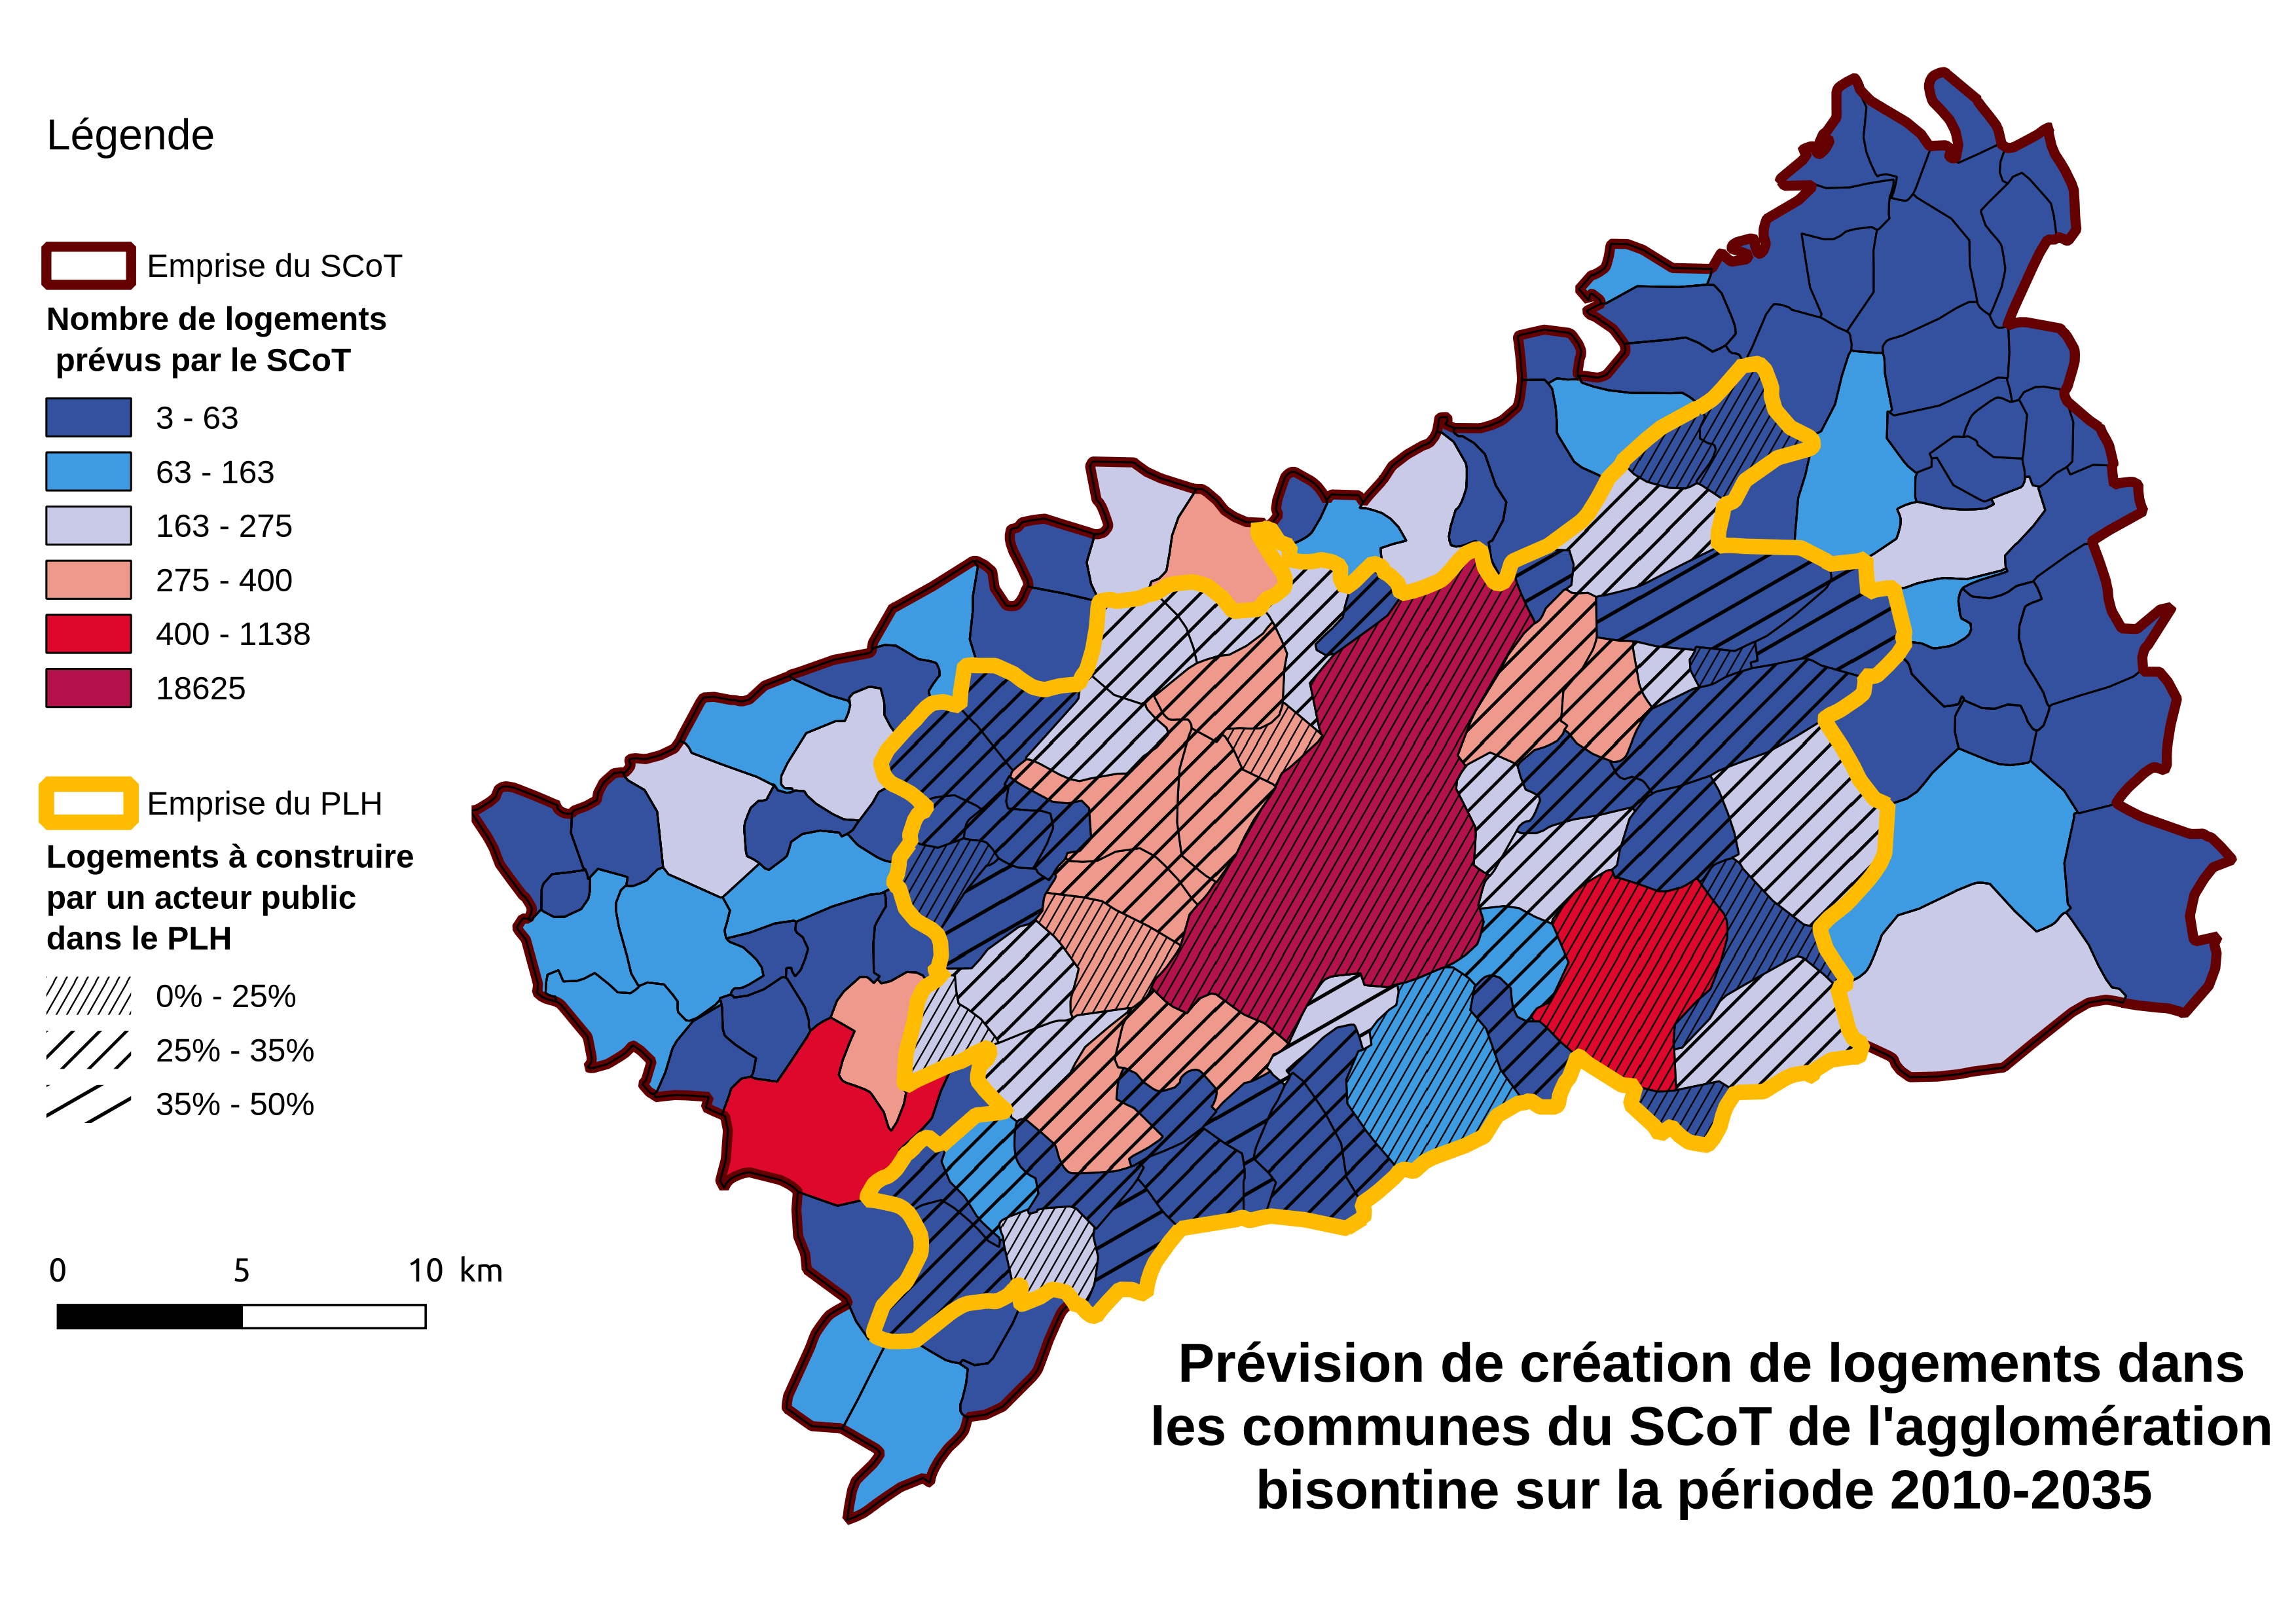
\includegraphics[width=11cm]{cartes/prevision-plh.png}
\end{frame}

\begin{frame}{Documents de planification locale - Les PLU}
Le \textbf{Plan Local de l’Urbanisme (PLU)} détaille et spatialise les contraintes de constructibilité au sein d’une commune
\begin{itemize}
\item a des \textbf{effets directs sur la constructibilité} mais ne planifie pas la construction 
\item \textbf{donne un cadre} pour la création de programmes de construction de logements \textit{(OAP, ZAC, ZAD)}
\item se compose en partie d'un \textbf{zonage} et d'un \textbf{règlement}
\end{itemize}
\end{frame}	

\begin{frame}{Application d'un PLU - Le zonage}
\begin{columns}[T]
\begin{column}[T]{7cm}
Zones générales et sous-zones particulières
\begin{itemize}
\item \alert{Naturelles} \textbf{(N)} \emph{non constructibles}
\item \alert{Agricoles} \textbf{(A)} \emph{non constructibles}
\item \alert{Urbanisées} \textbf{(U)}
\item \alert{À Urbaniser} \textbf{(AU)}
\end{itemize}
\end{column}
\begin{column}[T]{4cm}
\begin{textblock*}{6cm}(7.5cm,1.5cm)
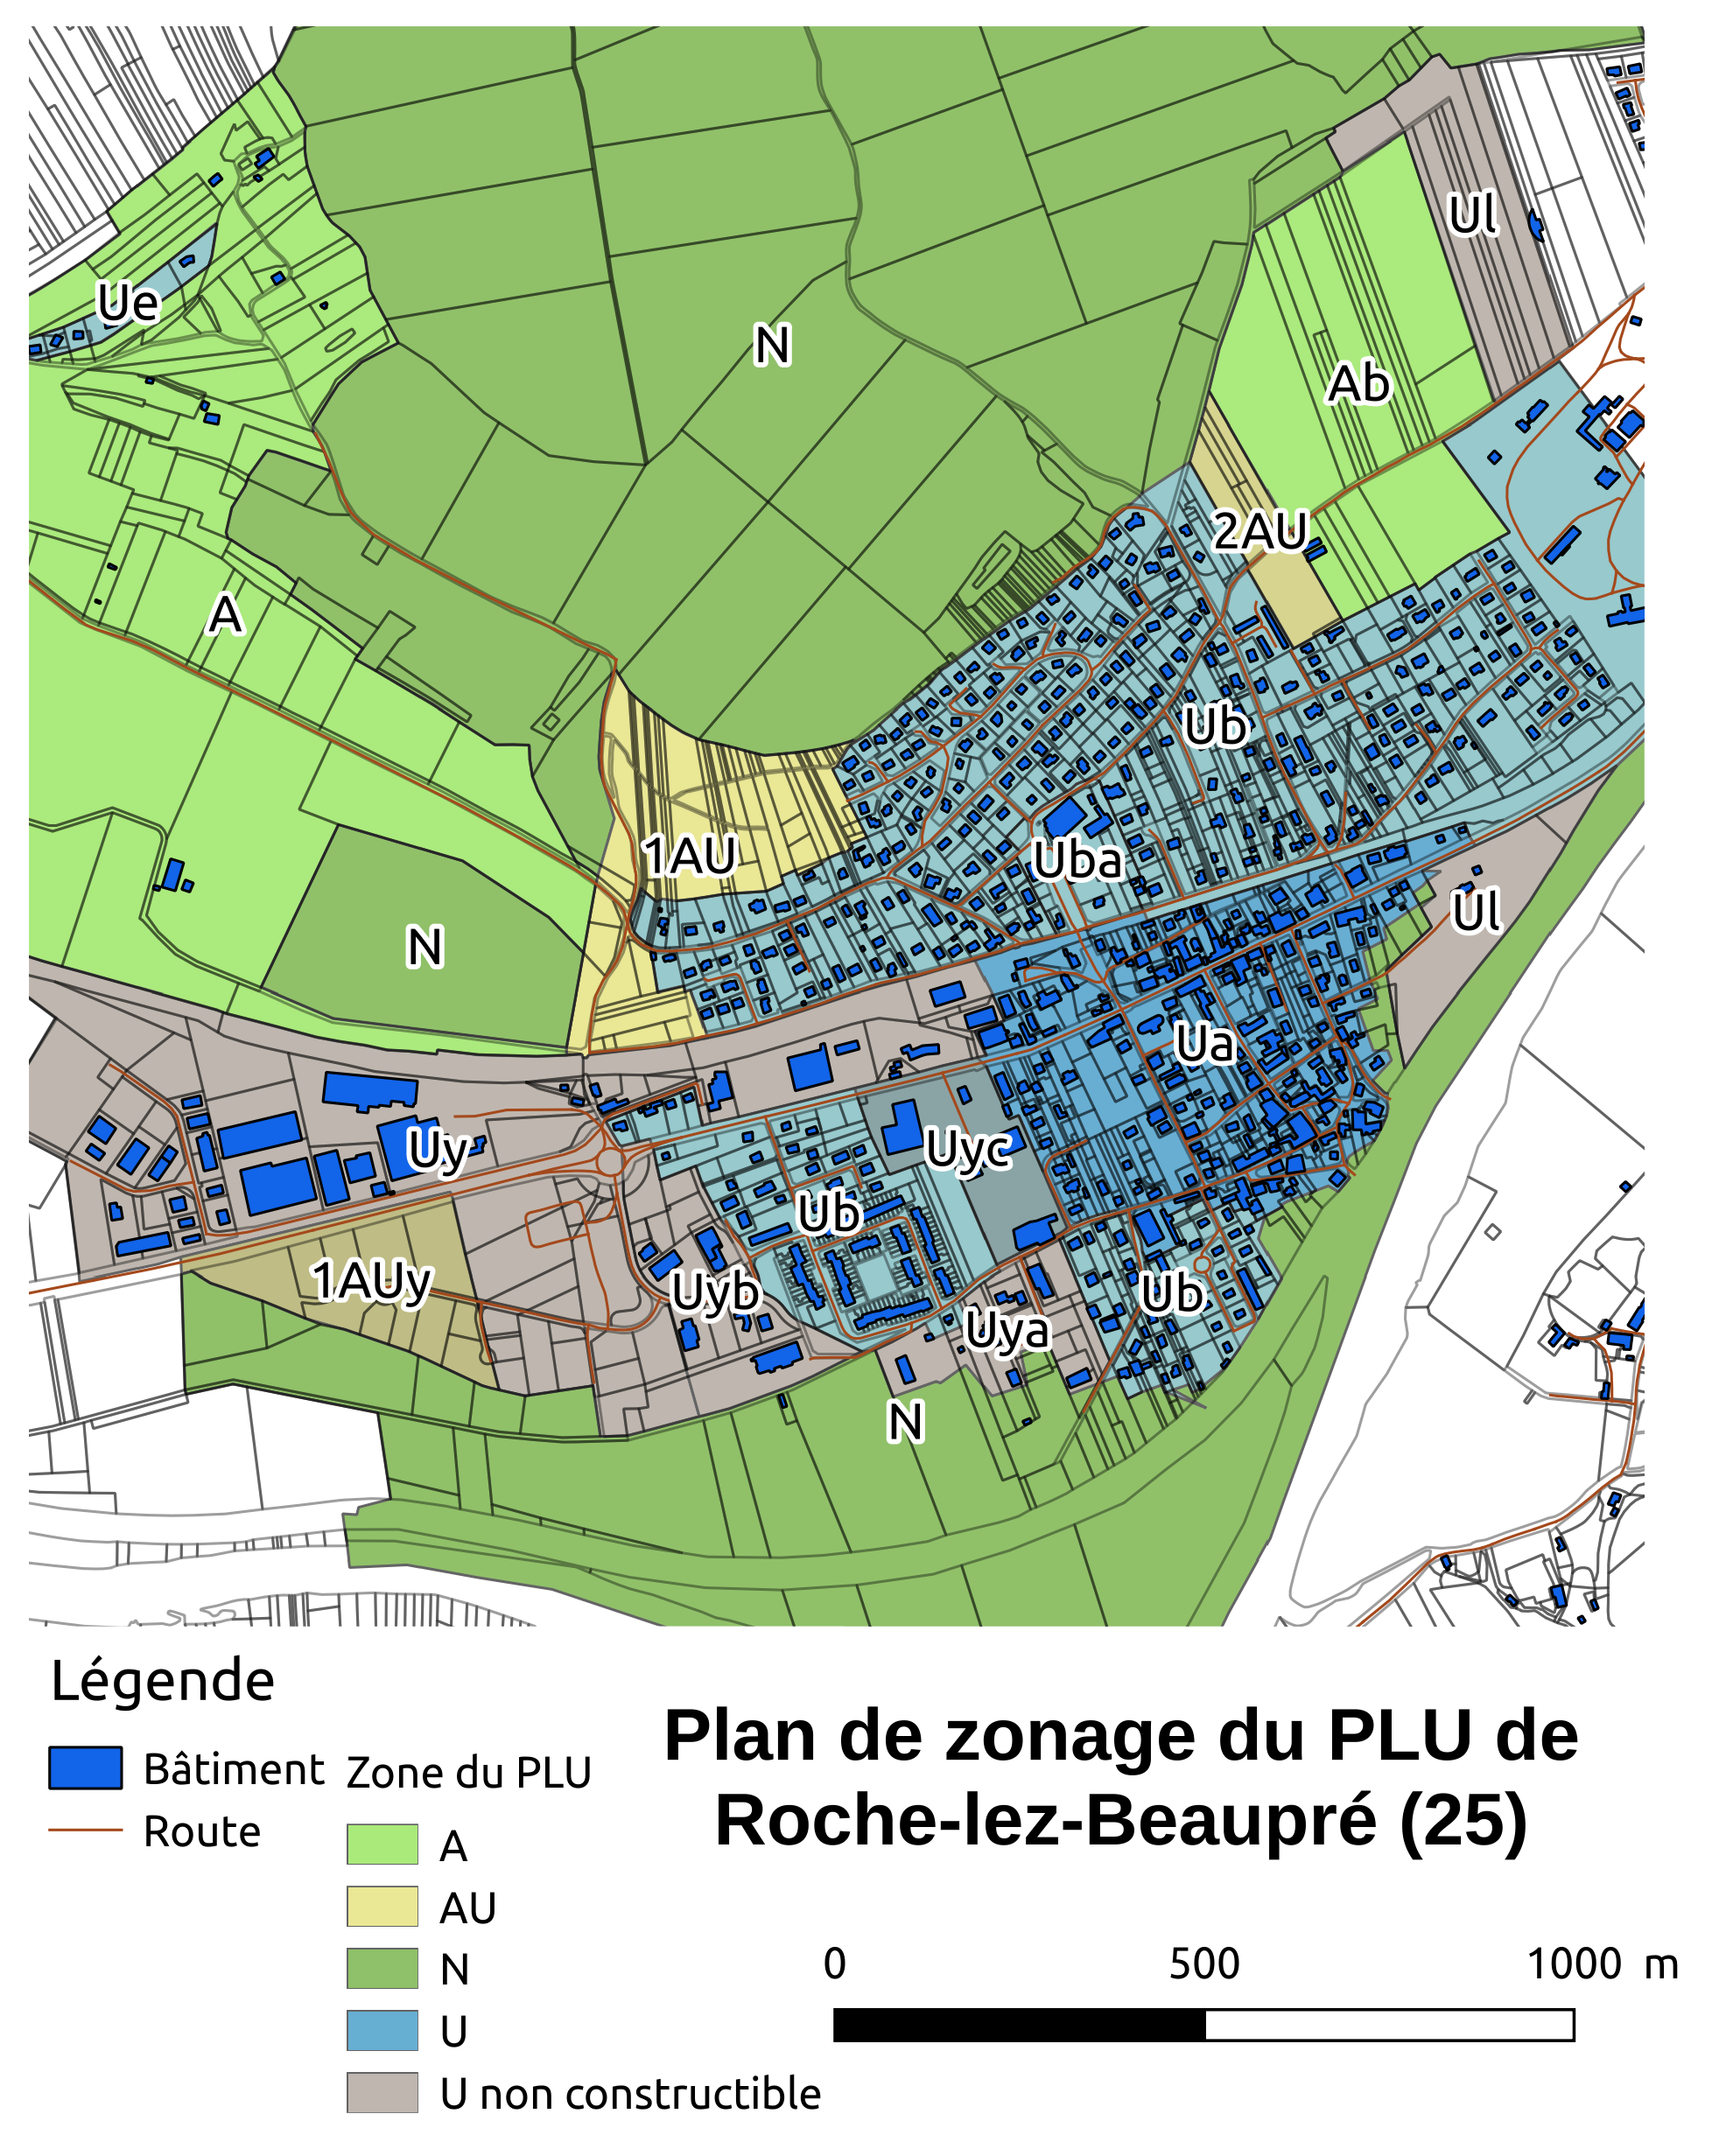
\includegraphics[width=5cm]{cartes/plu-roche.png}
\end{textblock*}	
\end{column}
\end{columns}

\end{frame}

\begin{frame}{Rétro action pour la compatibilité en modifiant le zonage}
	
\end{frame}

\begin{frame}{Application d'un PLU - Le règlement}
\begin{columns}[T]
\begin{column}[T]{5cm}
Pour chaque sous-zone : 
\begin{itemize}
\item Articles 1, 2 : restrictions d’\textbf{usage du sol}
\item Articles 6, 7, 8 : \textbf{position des bâtiments} relativement aux autres bâtiments, aux limites de parcelles ou à la voirie
\item Article 10 : \textbf{hauteur maximale}
\item Article 11 : \textbf{aspect extérieur}
\end{itemize}
\end{column}
\begin{column}[T]{5.5cm}
\centering
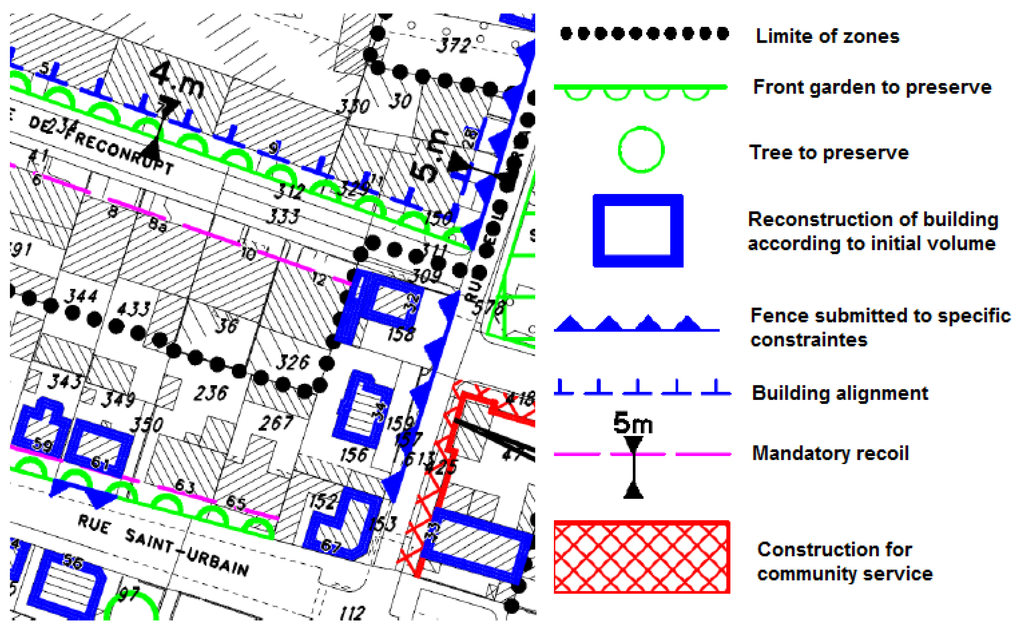
\includegraphics[width=6cm]{Images/codesplu.png}
\\
\textit{Exemple de prescriptions graphiques (PLU de Strasbourg)}
\end{column}
\end{columns}
\end{frame}

\begin{frame}{Opportunités pour l'IGN}
%	\centering{\includegraphics[width=4cm]{Images/franceGPU.png}}\\
%	\FontPetit{\textit{Dépôt des PLU sur le GPU}}
\begin{itemize}
	\item Définition de données adaptées à la simulation des évolutions
	\item Proposition de service aux acteurs de la planification sur l'ensemble du territoire français
	\item Certification de la robustesse du processus de simulation relativement à la qualité des données
\end{itemize}
\end{frame}